\documentclass{article}

\usepackage[ngerman]{babel}                % german translation for document elements
\usepackage{hyperref}                      % clickable links
\usepackage{amsmath, amssymb}              % mathe formeln
\usepackage{graphicx, caption, subcaption} % for figures and subfigures
\usepackage{float}                         % enforce figure placement

% ////////////////////////////////////////////////

%  @important
%  Für Publish den input kommentieren

\usepackage{xcolor}
\definecolor{mred}{HTML}{fe163d}
\definecolor{mgreen}{HTML}{009052}
\DeclareRobustCommand{\@todo(viktor):}[1]{\textcolor{mred}{@todo:} \textcolor{mred}{#1}} 
\DeclareRobustCommand{\at}[1]{\textcolor{mgreen}{#1}}


% ////////////////////////////////////////////////
% ////////////////////////////////////////////////

\title{Wave Function Collapse auf Graphen}
\author{
       Viktor Berengar Askan Graf von Westarp
    \\ \textit{FB5 Informatik und Sprachen}
    \\ \textit{HS Anhalt}
    \\ \texttt{viktor.grafvonwestarp@student.hs-anhalt.de}
}
\date{\today}

% ////////////////////////////////////////////////
\begin{document}

\@todo(viktor):{titelblatt ordentlich machen}
\\ \@todo(viktor):{Abbildungen an den richtigen orten inline erzwingen, figure placement parameter alle checken}
\\ \@todo(viktor):{\at{@translation} Collapsed und Observed als Begriffe vereinheitlichen}

\maketitle
\pagebreak

\tableofcontents
\pagebreak

% ////////////////////////////////////////////////
% ////////////////////////////////////////////////





\begin{abstract}
To be done.
\end{abstract}





\section{Einleitung}
    \subsection{Motivation}
    \subsection{Problemstellung und Ziel}
    \subsection{Problemlösung}
    \subsection{Aufbau der Arbeit}





\section{Hintergrund}
    \at{@incomplete Einleitender Satz, was zu prozeduraler Generierung}
    
    \subsection{Model Synthesis}
        Mit dem \textit{Model Synthesis} \cite{merrel} Algorithmus \ref{fig:ms_merrel} können, basiert auf einem 3D Beispielmodell, eine große Menge an ähnlichen 3D Modellen prozedural generiert werden (siehe Abbildung \ref{fig:ms_output}). Das synthesierte/generierte Model wird auf einem 3D Gitter iterativ generiert, indem jedem Knotenpunkt des Gitters ein Teil des Beispielmodells zugewiesen wird. Das Beispiel muss vorher in kleinere gleichgroße Bauteile zerlegt werden. Jedem Knotenpunkt wird zu Beginn die Menge aller Bauteile als seine Auswahlmöglichkeiten zugewiesen. Mit jeder Iteration wird bei einem Knotenpunkt ein Bauteil seiner Zustandsmenge ausgewählt. Danach werden alle Nachbarn geprüft, so dass sie nur noch passende Bauteile in ihrer Zustandsmenge behalten. Hierfür wird eine globale Suche verwendet, andere Methoden beschränkten sich zuvor nur auf lokale Suchen. Eine globale Suche ist besser, weil jedes Bauteil einen weitreichenden Einfluss auf das gesamte Gitter haben kann. 
        
        \begin{figure}[H]
    \centering
    \begin{minipage}{\linewidth}
        \rule{\linewidth}{0.4pt}
         
        \begin{enumerate}
        \item $M_0$ ist ein simples konsitentes Modell. $M = M_0$
        \subitem Wiederhole 2. bis 5. bis jeder Teil des Modells angepasst wurde
        \item Wähle eine Menge $B$ an Knotenpunkten zur Bearbeitung
        \item  $M' = M$ ohne die Knotenpunkte $B$ und deren bisherigen Bauteilen
        \item Arbeite alle Knotenpunkte von $B$ ab:
        \subitem Wähle einen Knotenpunkte aus und weise ihm ein konsistentes Bauteil zu
        \subitem Ist $M'$ nicht mehr konsistent, dann brich ab
        \subitem Füge diesen Knotenpunkt in $M'$ ein
        \item Wenn $M'$ noch konsistent ist, dann $M = M'$
        \end{enumerate}
        
        \rule{\linewidth}{0.4pt}
    \end{minipage}
    
    \caption{Model Synthesis Algorithmus nach Merrel \cite{merrel}}
    
    \label{fig:ms_merrel}
\end{figure}
        \begin{figure}[H]
    \centering
    \begin{subfigure}{0.18\textwidth} 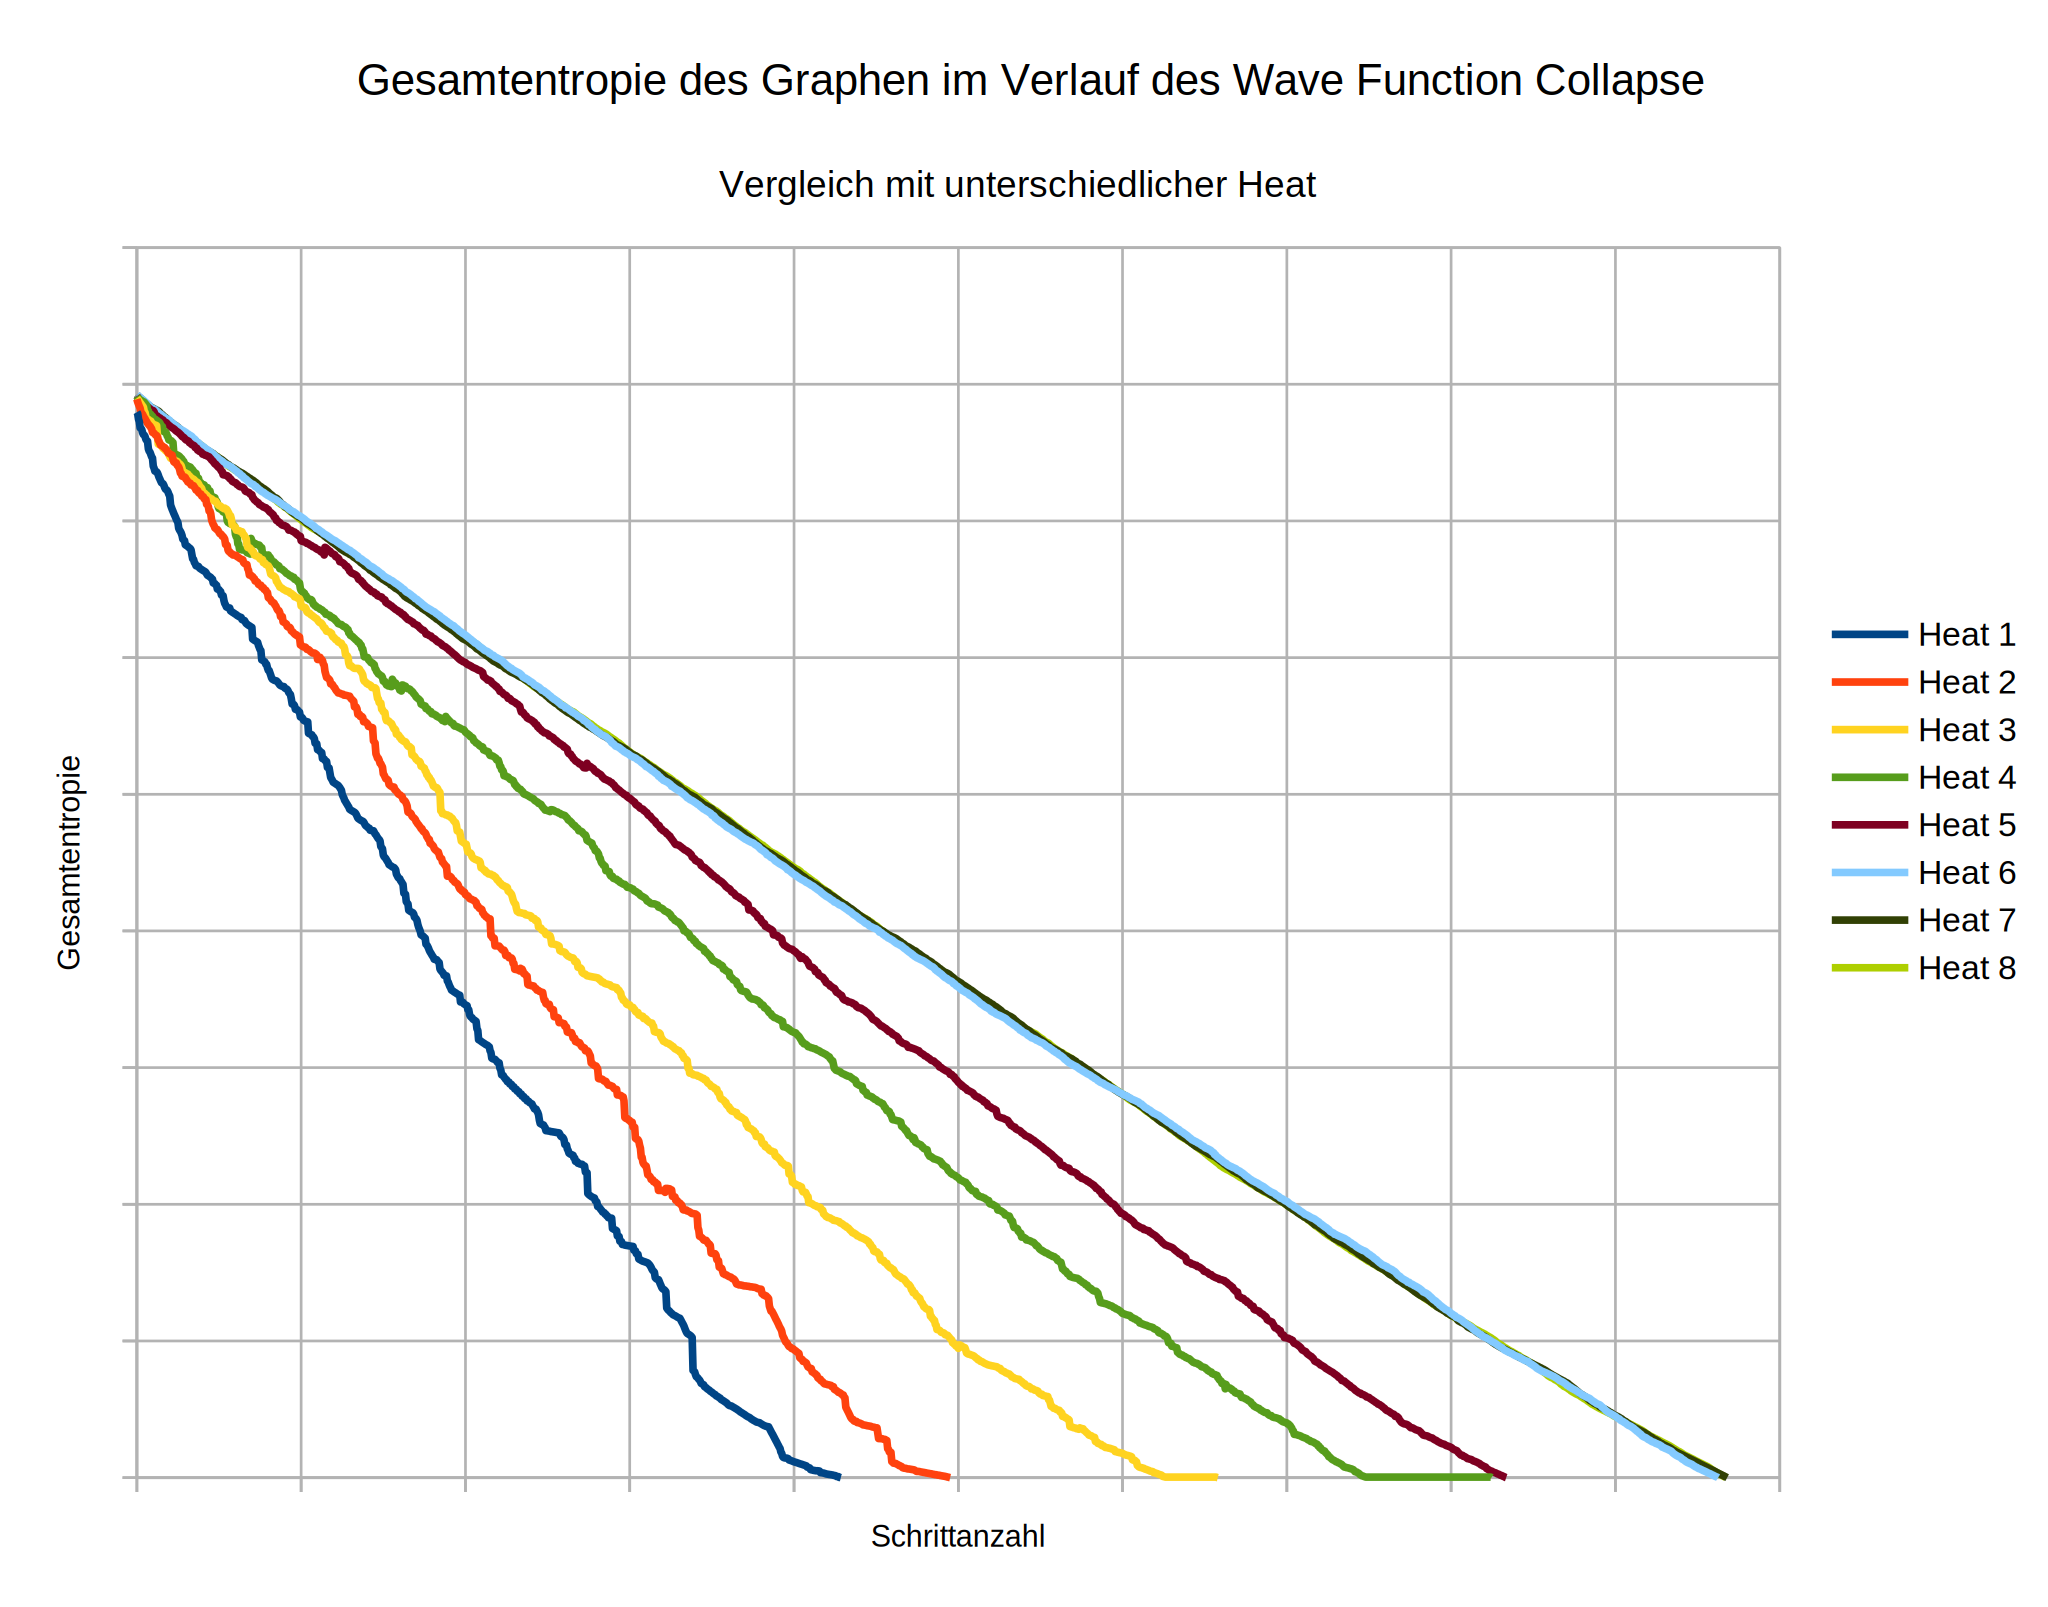
\includegraphics[width=\linewidth]{data/townscaper_grid/1.png} \caption{} \end{subfigure}
    \begin{subfigure}{0.18\textwidth} \includegraphics[width=\linewidth]{data/townscaper_grid/2.png} \caption{} \end{subfigure}
    \begin{subfigure}{0.18\textwidth} \includegraphics[width=\linewidth]{data/townscaper_grid/3.png} \caption{} \end{subfigure}
    \begin{subfigure}{0.18\textwidth} \includegraphics[width=\linewidth]{data/townscaper_grid/4.png} \caption{} \end{subfigure}
    \begin{subfigure}{0.18\textwidth} \includegraphics[width=\linewidth]{data/townscaper_grid/5.png} \caption{} \end{subfigure}
    
    \caption{
        Generierung eines Teils des Gitters für Townscaper \cite{stalberg_grid}. (a) Punkte werden generiert. (b) Triangulierung. (c) Kanten werden gelöscht, so dass Vierecke entstehen. (d) die Vierecke werden geviertelt. (e) Position der Knoten wird aufgelockert, so dass die Winkel zwischen Kanten gleichmäßiger sind.
    }
    \label{fig:townscaper_grid}
\end{figure}
        
        Damit die Ausgabe eine sinnvolle Anordnung der Bauteile ergibt, werden nur Bauteile die nebeneinander in einer bestimmten Richtung im Beispiel sind, in der Ausgabe nebeneinander in dieser Richtung platziert. Dadurch ist garantiert, dass jede kleine Region der Ausgabe mindestens einer Region im Beispiel gleicht. Da an jedem Knotenpunkt meist mehr als ein Bauteil passen würde und die Auswahl per Zufall geschieht, ist es unwahrscheinlich, dass die Ausgabe genau dem Beispiel im ganzen gleicht. Bei der Auswahl des Bauteils für einen Knoten wird die Wahrscheinlichkeit jedes Bauteils auch mit seiner Häufigkeit im Beispiel gewichtet, wodurch über eine große Menge an Ausgaben die Häufigkeit einzelner Bauteile der tatsächlichen Häufigkeit im Beispiel gleicht. Für eine einzelne Ausgabe bedeutet dies, dass die globale Verteilung der Bauteile auch tendenziell der Verteilung im Beispiel gleicht. 
        \at{@incomplete Vielleicht auch Resemblance und Consistency als konkrete Begriffe erklären}
        
        Die selbe Methodik kann auch auf 2D Gittern angewendet werden; dies wird dann \textit{Texture Synthesis} genannt. Desweiteren kann der Algorithmus um andere Techniken der prozeduralen Generierung erweitert werden, so können z.B. andere beliebige Beschränkungen auf die Ausgabe angewendet werden. \at{@visual}
        
        Die Ausgabe des Algorithmus kann auch durch Soft-Constraints beschränkt werden. Ebenso kann Symmetrie, Spiegelung und Drehung, in der Ausgabe erzwungen werden. Beide Ansätze wurden nicht weiter in dieser Arbeit betrachetet. Es wird empfohlen, dass der Algorithmus nicht das ganze Gitter auf einmal löst, damit Widersprüche nicht zu einem kompletten Neustart führen. Stattdessen sollen iterativ kleine Abschnitte für sich solange gelöst werden bis eine valide Ausgabe entsteht \ref{fig:ms_algorithm}. In dieser Arbeit wurde darauf verzichtet.
        
        \begin{figure}[H]
    \centering
    \begin{subfigure}{0.18\textwidth} 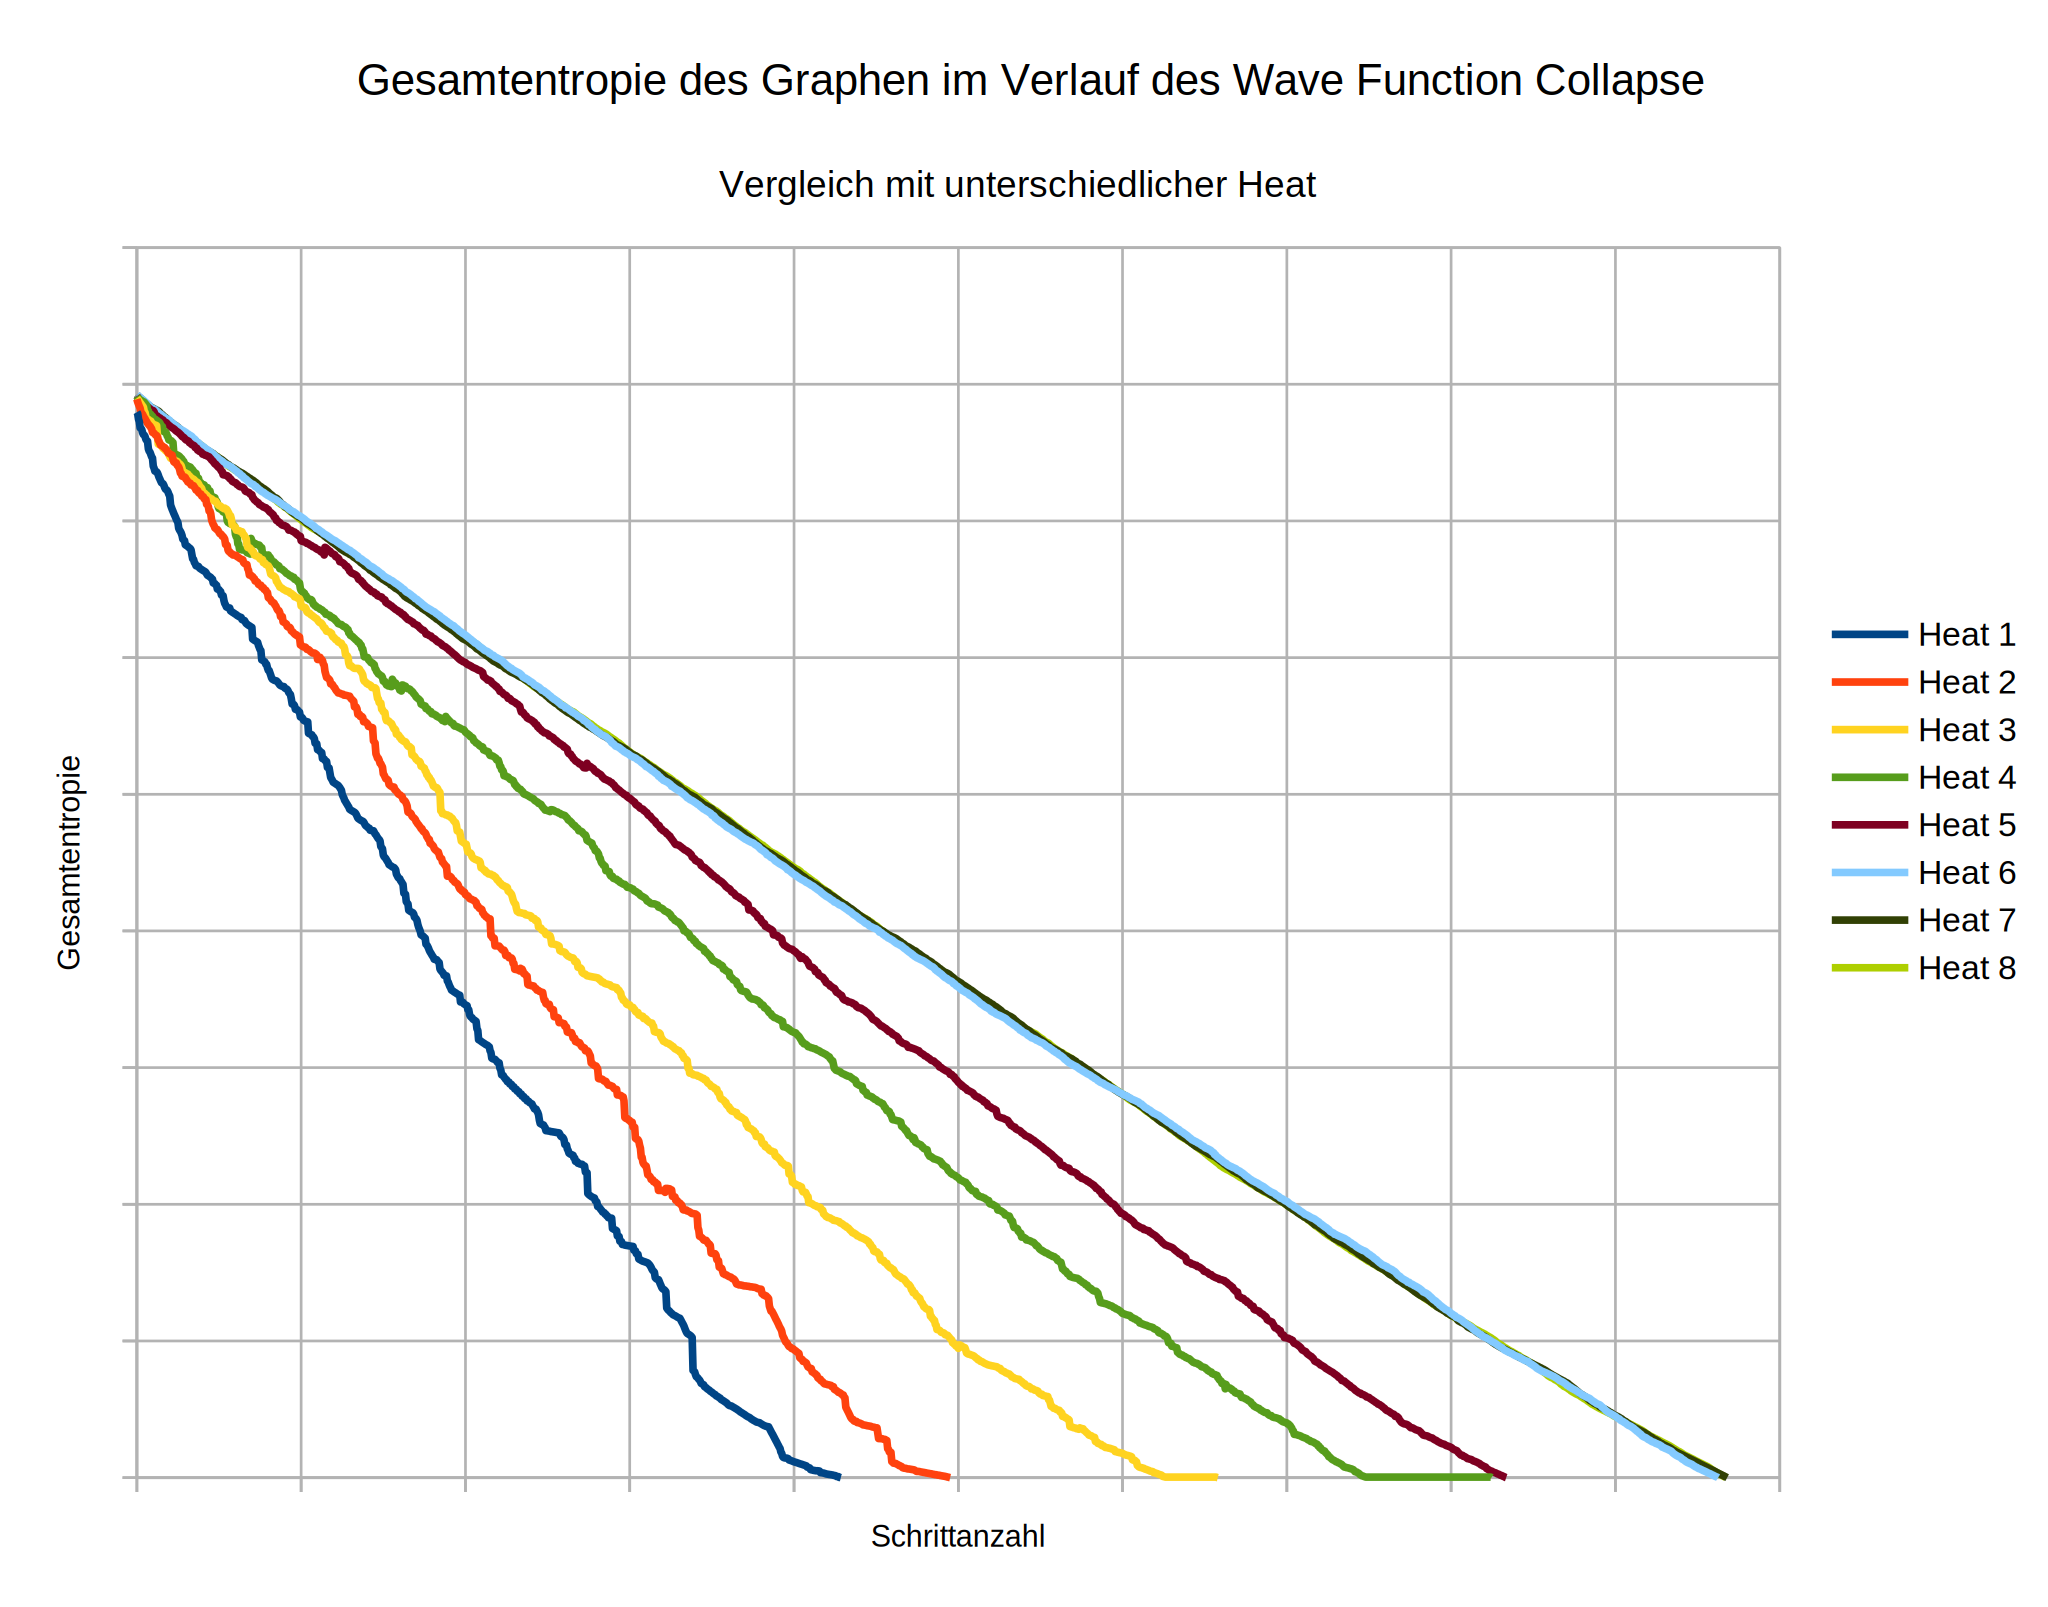
\includegraphics[width=\linewidth]{data/townscaper_grid/1.png} \caption{} \end{subfigure}
    \begin{subfigure}{0.18\textwidth} \includegraphics[width=\linewidth]{data/townscaper_grid/2.png} \caption{} \end{subfigure}
    \begin{subfigure}{0.18\textwidth} \includegraphics[width=\linewidth]{data/townscaper_grid/3.png} \caption{} \end{subfigure}
    \begin{subfigure}{0.18\textwidth} \includegraphics[width=\linewidth]{data/townscaper_grid/4.png} \caption{} \end{subfigure}
    \begin{subfigure}{0.18\textwidth} \includegraphics[width=\linewidth]{data/townscaper_grid/5.png} \caption{} \end{subfigure}
    
    \caption{
        Generierung eines Teils des Gitters für Townscaper \cite{stalberg_grid}. (a) Punkte werden generiert. (b) Triangulierung. (c) Kanten werden gelöscht, so dass Vierecke entstehen. (d) die Vierecke werden geviertelt. (e) Position der Knoten wird aufgelockert, so dass die Winkel zwischen Kanten gleichmäßiger sind.
    }
    \label{fig:townscaper_grid}
\end{figure}
        
    \subsection{Wave Function Collapse}
        \textit{Wave Function Collapse} ist eine Weiterentwicklung des Model Sythesis Algorithmus \cite{gumin}. Die Kernidee der Generierung mittels einem Beispiel bleibt und wird um drei Aspekte erweitert. Anstatt nur Bauteile nebeneinander anzuordnen, können nun auch überlappende Teile des Beispiels automatisch aus einem Beispiel extrahiert werden. In jeder Iteration wird die Zelle mit der niedrigsten Entropie zuerst betrachtet. Und bei Bauteil-basierten Beispielen werden Symmetrien von Bauteilen für eine kompaktere Definition ausgenutzt. Der Algorithmus ist in Abbildung \ref{fig:wfc_gumin} dargestellt. Abbildung \ref{fig:wfc_overview} zeigt ein paar Beispiele und mögliche Ausgaben.
        
        \begin{figure}[ht]
    \centering
    \begin{minipage}{\linewidth}
        \rule{\linewidth}{0.4pt}
        
        \begin{enumerate}
        \item Read the input bitmap and count NxN patterns.
        \subitem (optional) Augment pattern data with rotations and reflections.
        \item Create an array with the dimensions of the output (called ''wave'' in the source). Each element of this array represents a state of an NxN region in the output. A state of an NxN region is a superposition of NxN patterns of the input with boolean coefficients (so a state of a pixel in the output is a superposition of input colors with real coefficients). False coefficient means that the corresponding pattern is forbidden, true coefficient means that the corresponding pattern is not yet forbidden.
        \item Initialize the wave in the completely unobserved state, i.e. with all the boolean coefficients being true.
        \item Repeat the following steps: \begin{enumerate}
            \item Observation: \begin{enumerate}
                \item Find a wave element with the minimal nonzero entropy. If there is no such elements (if all elements have zero or undefined entropy) then break the cycle (4) and go to step (5).
                \item Collapse this element into a definite state according to its coefficients and the distribution of NxN patterns in the input.
            \end{enumerate}
            \item Propagation: propagate information gained on the previous observation step.
        \end{enumerate}
        \item By now all the wave elements are either in a completely observed state (all the coefficients except one being zero) or in the contradictory state (all the coefficients being zero). In the first case return the output. In the second case finish the work without returning anything.
        \end{enumerate}
        
        \rule{\linewidth}{0.4pt}
    \end{minipage}
    
    \caption{Wave Function Collapse Algorithmus nach Gumin \cite{gumin}}
    
    \label{fig:wfc_gumin}
\end{figure}
        \begin{figure}[H]
    \centering
    \begin{subfigure}{0.18\textwidth} 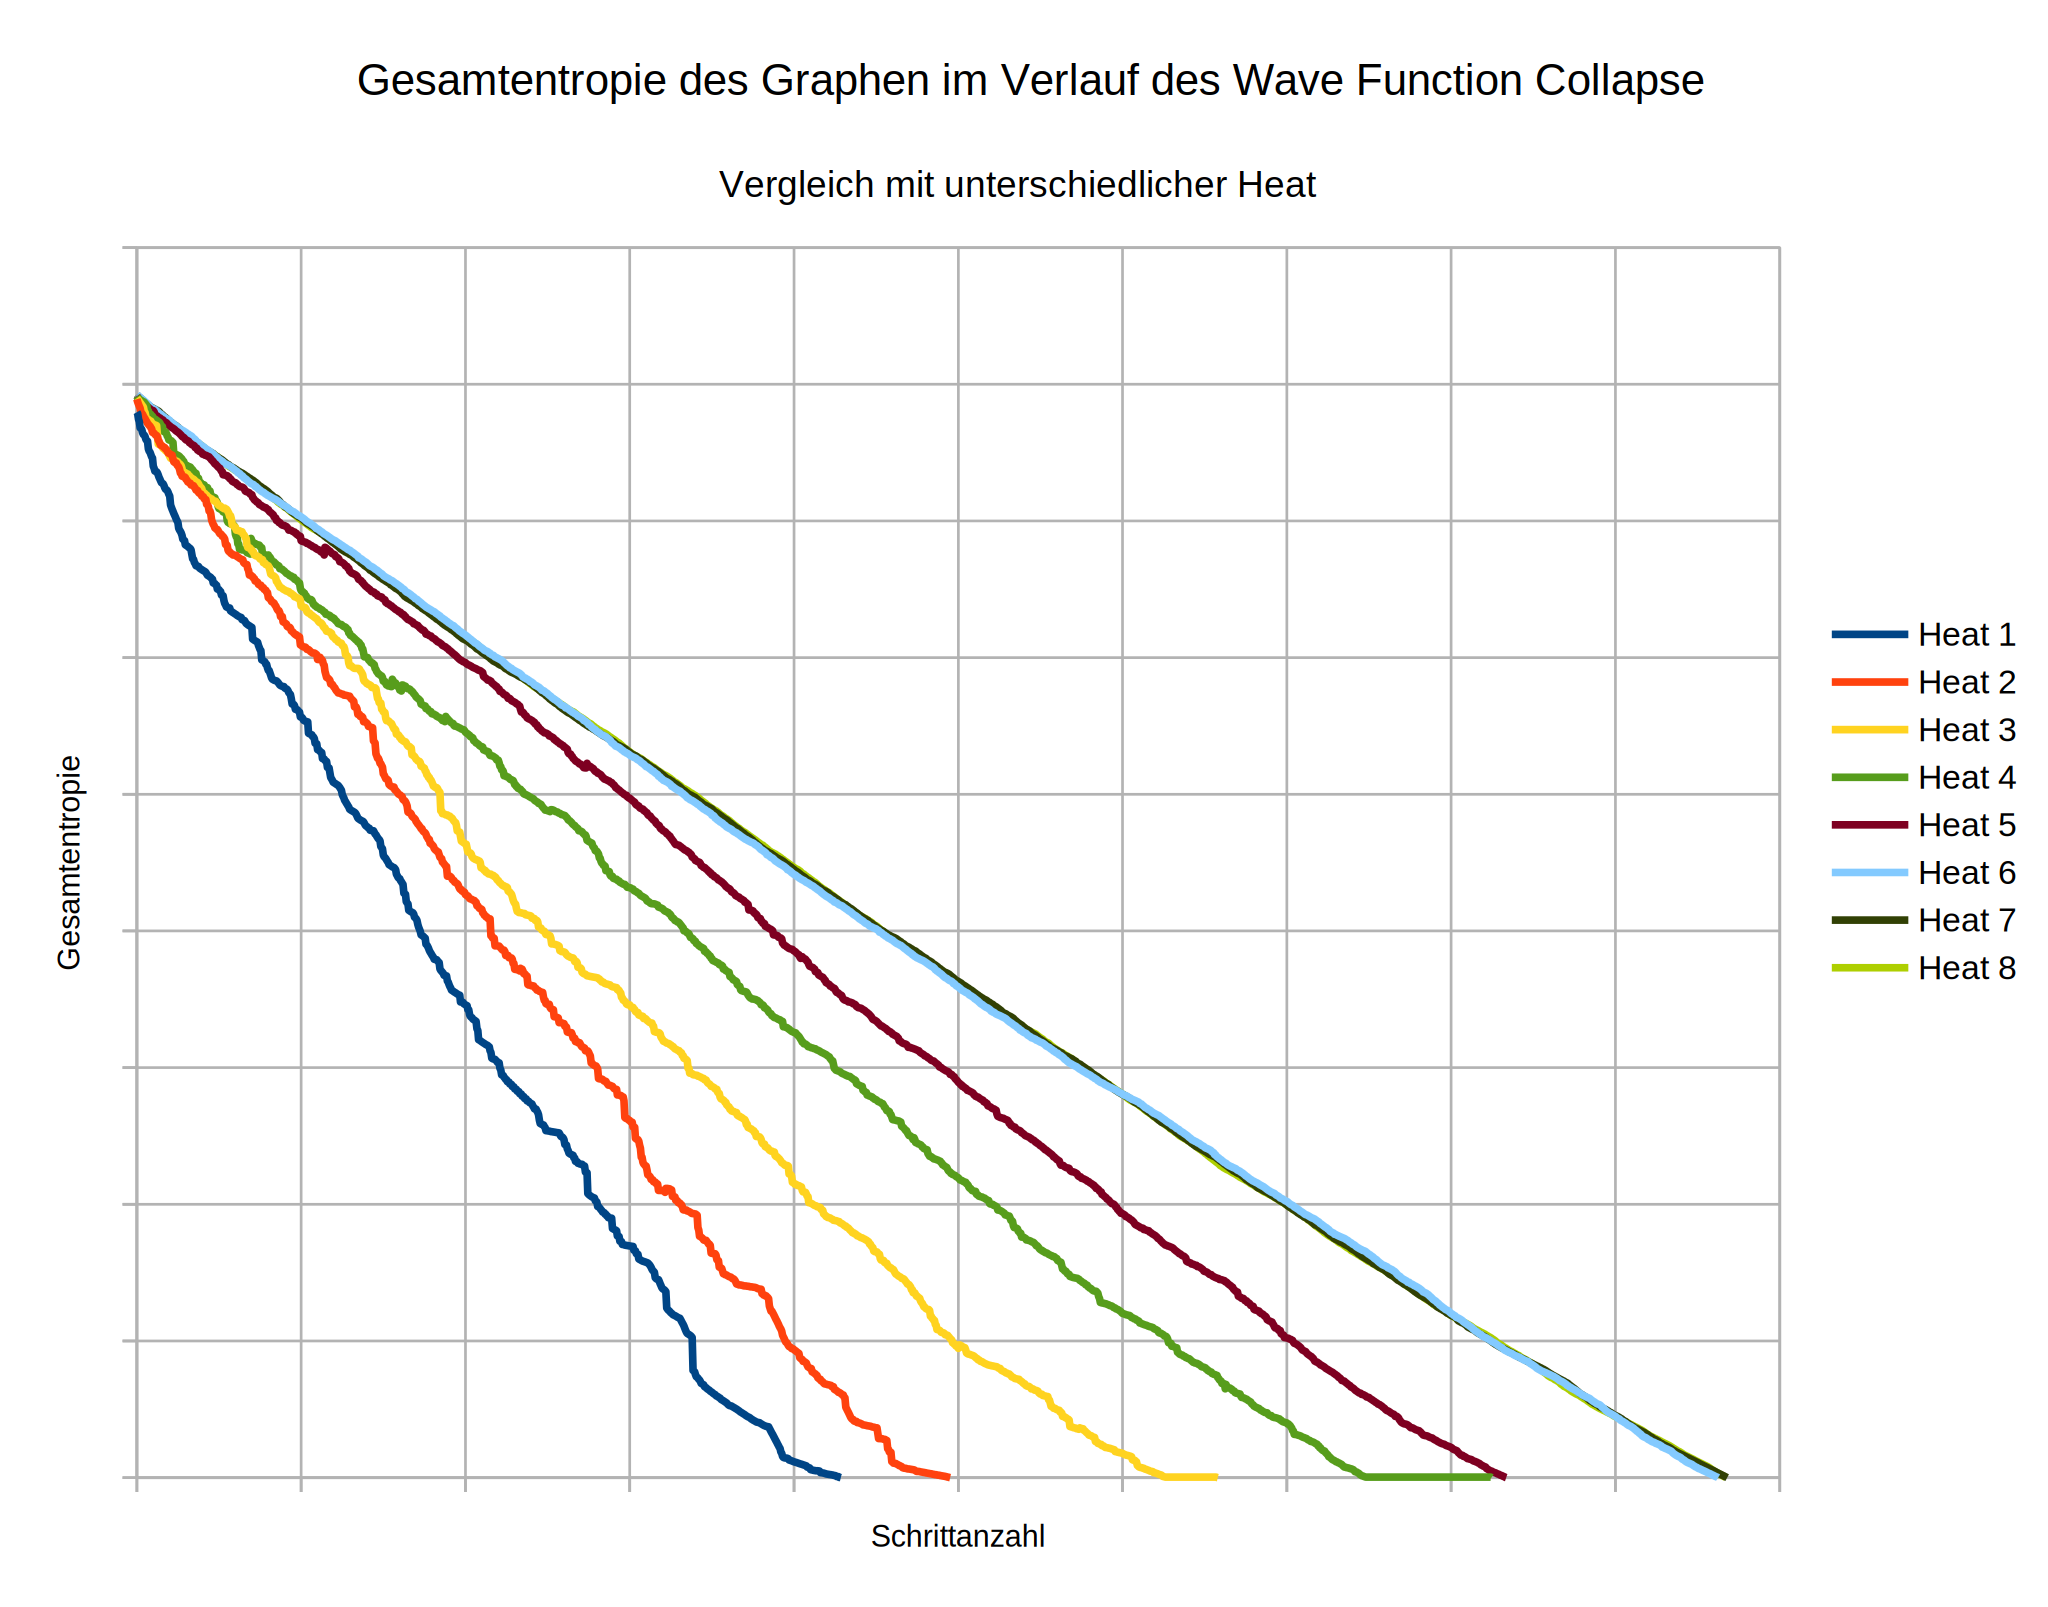
\includegraphics[width=\linewidth]{data/townscaper_grid/1.png} \caption{} \end{subfigure}
    \begin{subfigure}{0.18\textwidth} \includegraphics[width=\linewidth]{data/townscaper_grid/2.png} \caption{} \end{subfigure}
    \begin{subfigure}{0.18\textwidth} \includegraphics[width=\linewidth]{data/townscaper_grid/3.png} \caption{} \end{subfigure}
    \begin{subfigure}{0.18\textwidth} \includegraphics[width=\linewidth]{data/townscaper_grid/4.png} \caption{} \end{subfigure}
    \begin{subfigure}{0.18\textwidth} \includegraphics[width=\linewidth]{data/townscaper_grid/5.png} \caption{} \end{subfigure}
    
    \caption{
        Generierung eines Teils des Gitters für Townscaper \cite{stalberg_grid}. (a) Punkte werden generiert. (b) Triangulierung. (c) Kanten werden gelöscht, so dass Vierecke entstehen. (d) die Vierecke werden geviertelt. (e) Position der Knoten wird aufgelockert, so dass die Winkel zwischen Kanten gleichmäßiger sind.
    }
    \label{fig:townscaper_grid}
\end{figure}
        
        Der Name Wave Function Collapse ist eine Anspielung auf die Quantenphysik. So könnte man Quantenpartikel in Superposition mit den Zellen des Gitters vergleichen. Die Zellen haben auch mehrere mögliche finale Zustände bis sie observiert werden und in einen festen Zustand collapsen. Mathematisch besteht aber keine Beziehung. Auch werden andere Begriffe wie z.B. Knoten zu Zelle umbenannt und das Gitter als Wave bezeichnet.
        
        \at{@incomplete generalization to NxN Überlappung}
        
        Die Reihenfolge in der die Zellen observiert werden, hat einen Einfluss auf die Laufzeit. Bei Model Synthesis werden Zellen einfach nach ihrer Reihenfolge im Gitter abgearbeitet. Der Vorteil ist, dass keine Suche der nächsten Zelle nötig ist, aber es hat zum Nachteil, dass die Ausgabe sichtbare Artefakte enthällt. Man kann erkennen, ob zuerst die Reihen oder erst die Spalten abgearbeitet wurden. In Abbildung \ref{fig:directional_bias} wird der Unterschied zwischen den beiden Herangehungsweisen dargestellt. Wäre bekannt welche Zelle den meisten Fortschritt zur Lösung und die geringste Chance auf einen Widerspruch birgt, könnte stets diese Zelle zuerst betrachtet werden. Doch Merrel zeigt im Anhang seines Papers \cite{merrel}, dass die Entscheidung, ob eine Ausgabe vervollständigt werden kann, ein NP-vollständiges Problem ist. 
        
        \begin{figure}[H]
    \centering
    \begin{subfigure}{0.18\textwidth} 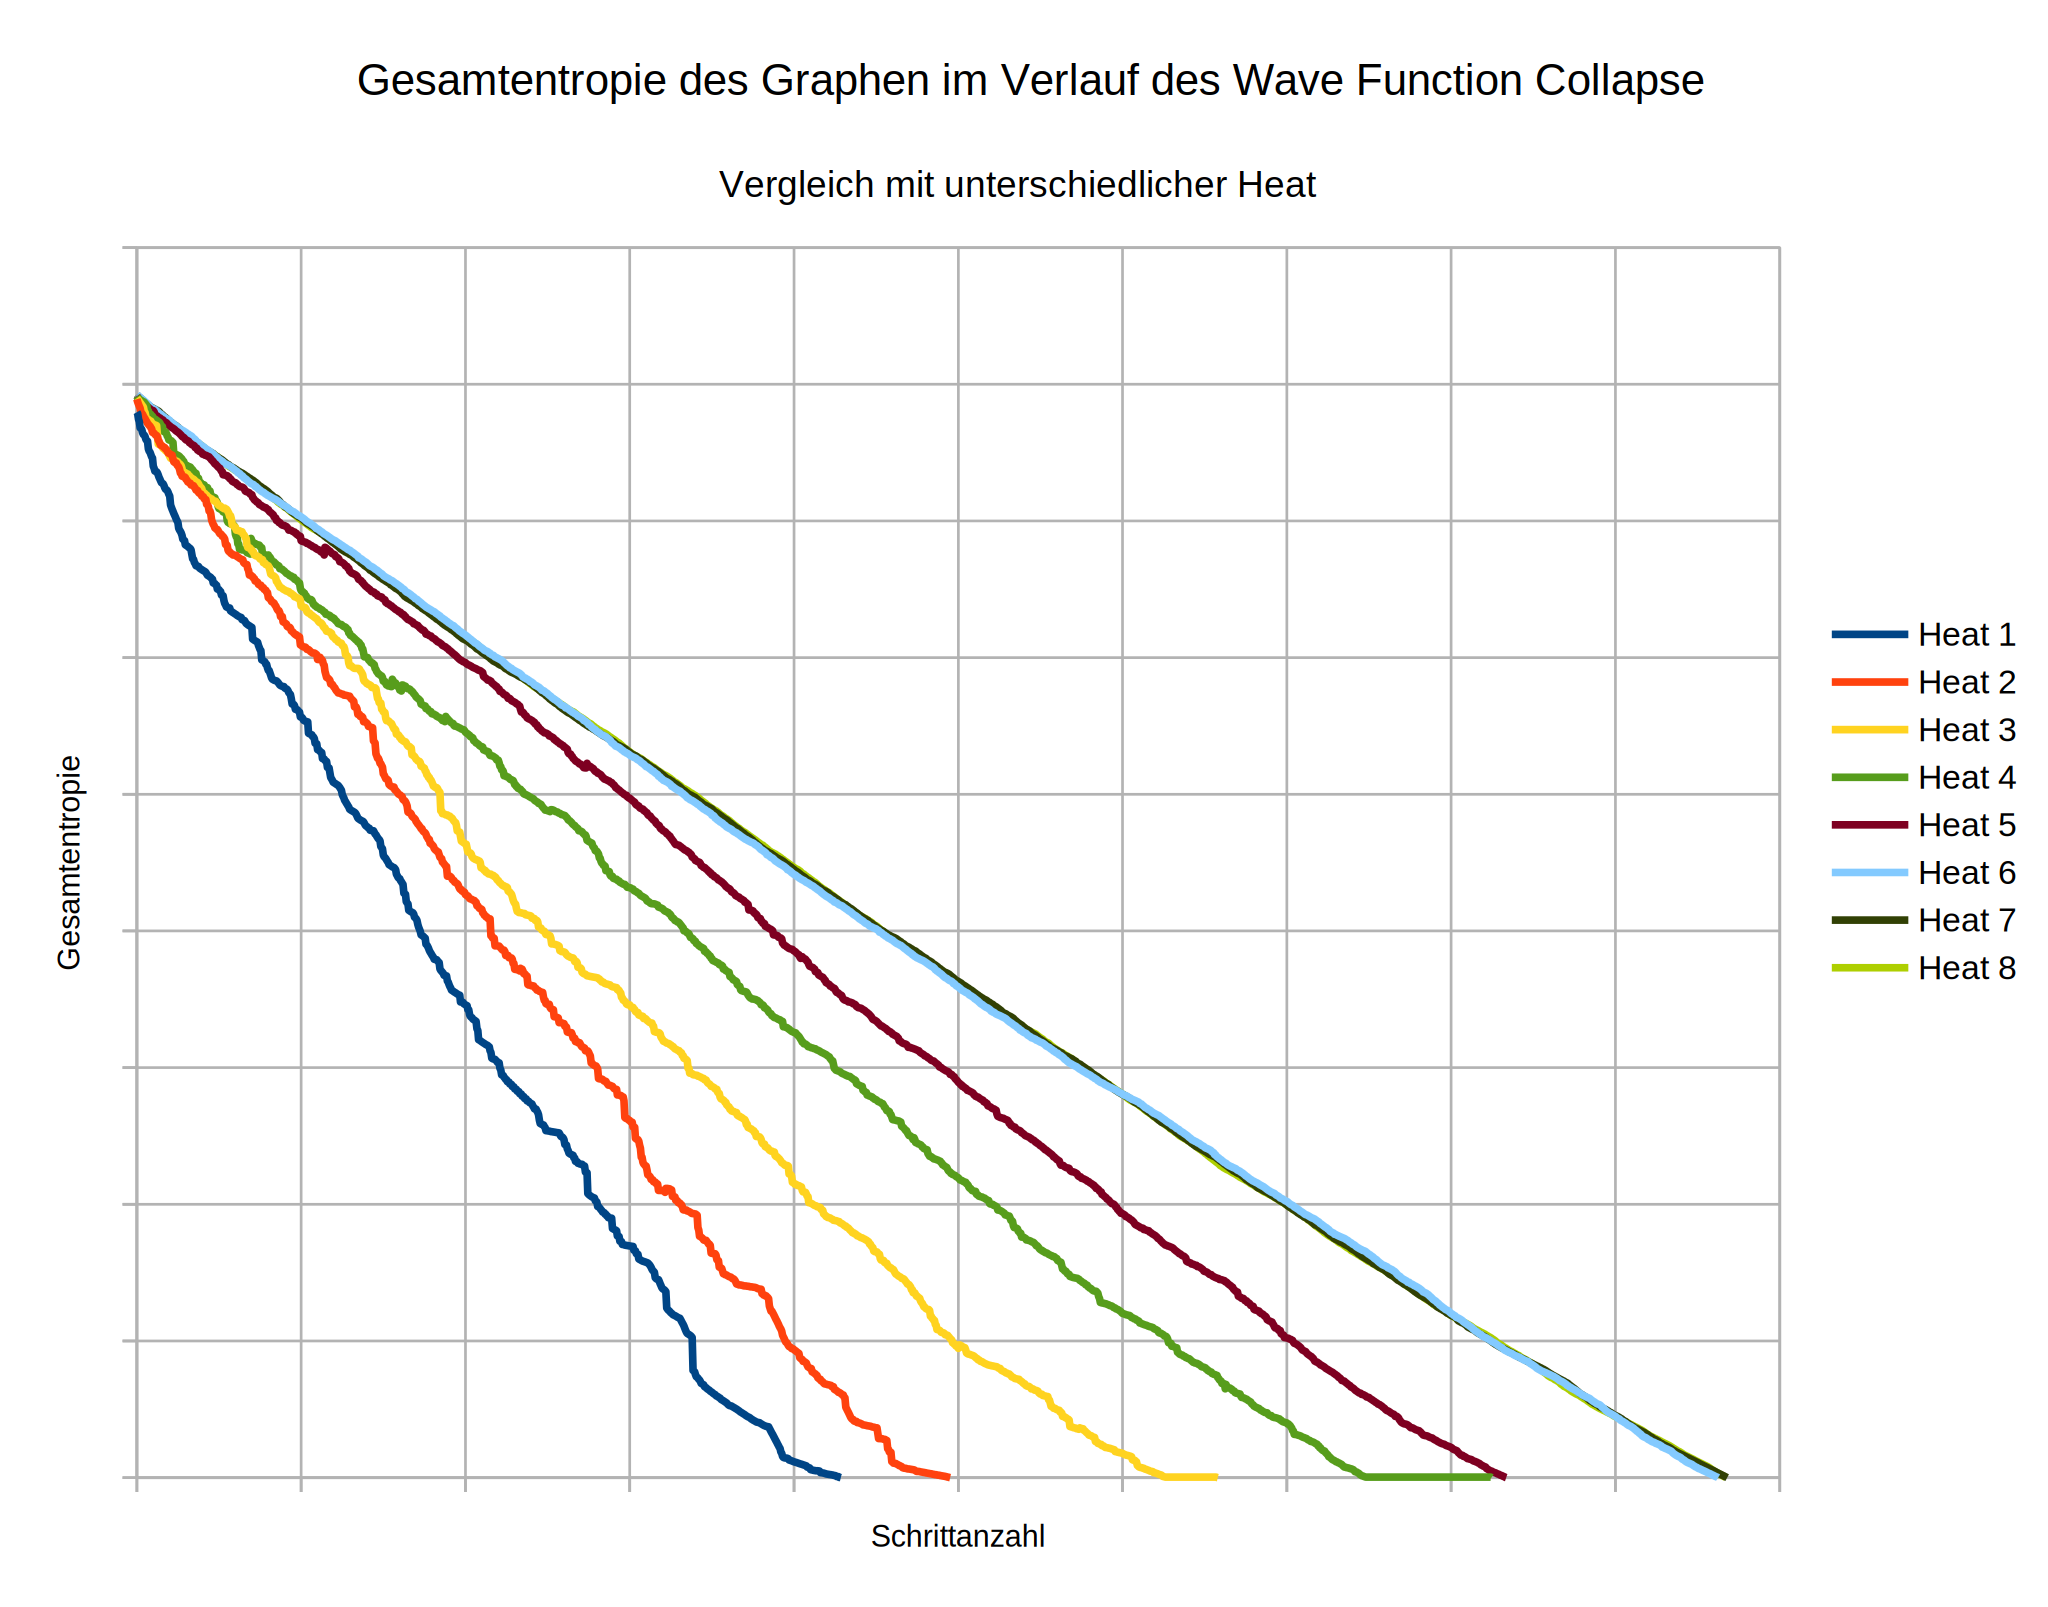
\includegraphics[width=\linewidth]{data/townscaper_grid/1.png} \caption{} \end{subfigure}
    \begin{subfigure}{0.18\textwidth} \includegraphics[width=\linewidth]{data/townscaper_grid/2.png} \caption{} \end{subfigure}
    \begin{subfigure}{0.18\textwidth} \includegraphics[width=\linewidth]{data/townscaper_grid/3.png} \caption{} \end{subfigure}
    \begin{subfigure}{0.18\textwidth} \includegraphics[width=\linewidth]{data/townscaper_grid/4.png} \caption{} \end{subfigure}
    \begin{subfigure}{0.18\textwidth} \includegraphics[width=\linewidth]{data/townscaper_grid/5.png} \caption{} \end{subfigure}
    
    \caption{
        Generierung eines Teils des Gitters für Townscaper \cite{stalberg_grid}. (a) Punkte werden generiert. (b) Triangulierung. (c) Kanten werden gelöscht, so dass Vierecke entstehen. (d) die Vierecke werden geviertelt. (e) Position der Knoten wird aufgelockert, so dass die Winkel zwischen Kanten gleichmäßiger sind.
    }
    \label{fig:townscaper_grid}
\end{figure}
        
        Einfacher ist es eine Heuristik zu definieren, die simpel zu berechnen ist und meistens einen besseren Ansatz bietet. Hierfür wird die Entropie als Maß eingeführt. Sie beschreibt das Maß an Ungewissheit über den finalen Zustand einer Zelle. Ist eine Zelle observiert, hat sie nur noch einen Zustand und die Entropie ist minimal, während eine Zelle mit vielen Möglichkeiten eine hohe Entropie hat. Die Entropie gibt auch Information darüber wie sehr eine Zelle durch ihre Umgebung beschränkt wird. Sie wird mit der Formel der Shannon-Entropie \cite{shannon} berechnet. 
        
        %     % \caption{
%     %     Formel für die Shannon-Entropie. 
%     %     $\mathcal{X}$ ist die Menge der Möglichen Zustände einer Zelle.
%     %     $p(x)$ ist die Wahrscheinlichkeit das $x$ gewählt wird.
%     % }

\begin{equation}
    \label{eq:entropy}
    \mathrm{entropy}(\mathcal{X}) = -\sum_{x \in \mathcal{X}} p(x),\log p(x)
\end{equation}
        
        Der Zerteilung eines Beispiels in Bauteile muss manuell passieren. Soll nun ein Bauteil auch in einer anderen Orientierung oder Spiegelung in der Ausgabe vorkommen müssen diese Variationen explizit angelegt werden. Will man nun ein Bauteil leicht verändern, so muss man auch alle Variationen manuel anpassen. Um diesen aufwendigen Prozess zu automatisieren definiert Gumin eine Gruppe von Symmetriearten mit denen eine Nutzerin ihre Bauteile annotieren kann. Der Algorithmus erkennt diese Annotationen und generiert vor Beginn automatisch die Variationen. Da sich diese Arbeit nicht mit Beispielen aus Bauteilen befässt, bleibt dieser Aspekt ungenutzt.
    
    
    \subsection{Gitter, Graphen, Triangulierung, Voronoi}
    
        \at{@incomplete Definition von Gitter und Graph in dieser Arbeit}
        
        \url{https://en.wikipedia.org/wiki/Delaunay_triangulation}\\
        \url{https://en.wikipedia.org/wiki/Voronoi_diagram}\\
        \url{https://de.wikipedia.org/wiki/Polygonnetz}\\
        \url{https://en.wikipedia.org/wiki/Triangulated_irregular_network}\\
        \url{https://en.wikipedia.org/wiki/Lattice_graph}\\
        
        \subsubsection{Gitter}
        \subsubsection{Graphen}
        \subsubsection{Triangulierung, Quadrilierung}
        \subsubsection{Delaunay Triangulation}
            \begin{itemize}
            \item Defintion der Triangulierung
            \item \at{@visual}
            \end{itemize}
        \subsubsection{Voronoi Diagramm}
            \begin{itemize}
            \item Definition
            \item nützliche Eigenschaften
            \end{itemize}





\section{Wave Function Collapse auf Graphen}
    In diesem Abschnitt wir dargestellt wie der Wave Function Collapse Algorithmus erweitert wird, so dass die Ausgabe nicht nur auf einem Gitter von Zellen geschehen kann, sondern auch auf Zellen mit freier Anordnung und Verteilung, einem Graphen, arbeiten kann. Es wird erklärt welche Aspekt des Algorithmus angepasst werden und welche beibehalten werden können. Desweiteren wird ein neues Konzept names \textit{Heat} eingeführt, welches dem Nutzer erlaubt die erzielte Ähnlichkeit zum Beispiel zu verringern um die Erfolgschance des Algorithmus zu verbessern.
    
    \subsection{Beschränkung des Wave Function Collapse und Idee zur Erweiterung}
        \@todo(viktor):{titel hat einen umbruch}
        
        Die ursprüngliche Form des Wave Function Collapse nimmt ein 2D Pixelmuster oder Tilesets als Beispiel und produziert darauß wieder 2D Muster. 
        Pixel liegen stets auf einem quadratischen Gitter. Bei Tilesets ist die grafische Gestaltung des Tiles zwar uneingeschränkt, dennoch sind die Tiles selbst quadratisch. Dies schränkt die Gestaltung des Inhalts der Tiles in sofern ein, dass die Kanten zu anderen Kanten passen müssen. Auch bei 3D Beispielen werden die Modelle in blockförmige Bauteile zerschnitten, damit der Collapse auf einem 3D Gitter von Würfeln arbeiten kann.
        
        Solche Gitter bringen bestimmte Vorteile durch ihre Struktur mit sich. Die Benachbarung von Zellen ist implizit aus dem Gitter erkennbar, die Nachbarzellen befinden sich stets in festen Abständen in die vier Himmelsrichtungen im 2D Gitter und entlang der drei Achsen, also 6 Richtungen, im 3D Gitter. Die Überlappungsregeln aus dem Beispiel können also direkt von dem einem Gitter auf das andere übertragen werden. Der Nachteil solcher Gitter ist, dass die Ausgabe, im Ganzen, Artefakte des Gitter aufweist. Nur vertikale und horizontale Linien können im Pixelgitter exakt dargestellt werden, frei geformte Kurven oder organische Strukturen lassen sich nur durch Annäherung darstellen und es kann zu Aliasing kommen.
        
        Im Kern des Wave Function Collapse wird geprüft, dass nur Zustände gewählt werden, die mit der Ausgabe bis dahin überlappen könnten. Die möglichen Überlappungen hängen dabei von der Richtung zwischen den Zellen ab. In einem Gitter kann jede Richtung zu einer Nachbarzelle aus dem Beispiel extrahiert werden. Wird die Anordnung und Benachbarung der Zellen nun aber vom Gitter gelöst, so ist es nicht mehr garantiert, dass die Richtungen zwischen Nachbarzellen auch im Beispiel existieren, stattdessen muss eine Funktion zur Übersetzung der tatsächlichen Richtung zu einer der extrahierbaren Richtungen definiert werden. Danach kann der Algorithmus wie zuvor mit den Überlappungen arbeiten um nun den Graphen zu befüllen.
    
    
    \subsection{Von Gittern zu Graphen}
        Ursprünglich arbeit Wave Function Collapse nur auf Gittern. Der Schritt zum Graphen als Fundament für die Ausgabe des Algorithmus ist sinnvoll, da Gitter eine spezielle Art von Graphen darstellen. In dem Umfang dieser Arbeit werden aber auch nicht alle Arten von Graphen betrachtet, meistens ist die freie Anordnung und Verbindung von Knoten nicht notwendig. Da jede Kanten eines Gitters zuvor eine lokale Benachbarung dargestellt haben und die Regelextrahierung nur lokal arbeitet, beschränkt sich diese Arbeit nur auf Graphen in denen Kanten auch primär einen Knotenpunkt mit den Knotenpunkten in einem lokalen Umfeld verbindet. \at{@visual Gitter und Graph des Gitters} Der Algorithmus kann auch auf anderen Arten von Graphen angewendet werden, doch können daraus neue oder unerwartete Effekte hervortreten, die wiederum anderen Lösungswege benötigen.
        
        Ein Gitter bringt mit sich Information über Benachbarung und Position jeder Zelle die nun auf einem Graphen explizit angegeben werden müssen. Je nach Anordnung kann nun nicht nur die Richtung zur Nachbarzelle sondern auch deren Abstand und die Anzahl an Nachbarzellen variieren. Bevor der Algorithmus eine Ausgabe generieren kann, müssen diese Information vom Nutzer angegeben werden.
        
        Jede Kante des Graphen stellt eine Beschränkung des Lösungsraums dar. Bei einem Gitter ist jede Zelle, mit Ausnahme der Zellen am Rand, gleichermaßen beschränkt, jedoch kann die Anordnung des Graphen dazu führen dass einzelne Zelle weniger und andere stärker eingeschränkt werden. Eine Zelle mit zehn Nachbarn muss in einen Zustand collapsen, welcher zu den Zuständen der zehn Nachbaren passt. Ein Graph kann somit stark beschränkte und schwach beschränkte Regionen enthalten, während dass Gitter uniforme Beschränkung auf Zellen ergibt. Zur Erinnerung: es muss nur eine Zelle eine Widerspruch verursachen damit der Algorithmus fehlschlägt. Also sind solche Regionen starker Beschränkung besonderns entscheident für die Chance eine valide Ausgabe zu generieren, weil hier der Lösungsraum am kleinsten ist.
        
        \at{@incomplete Entropie(höhere Entropie durch Heat) erwähnen und für Regionen mit einer Grafik von der App darstellen}
    
    
    \subsection{Regelextraktion}
        \at{@flow Die Absätze sind okay aber ihre Reihenfolge muss überdacht werden}
        \at{@incomplete Diagonale Regeln, besseres Sampling des Beispiels}
        
        Ziel des Wave Function Collapse ist es, eine große Anzahl lokal ähnlicher Ausgaben zu generieren. Ähnlichkeit wird erreicht, wenn jede kleine Region der Ausgabe zu Regionen des Beispiels passt. Der Algorithmus weist jeder Zelle des Graphen einen Zustand zu, so dass zwei Bedingungen gelten. Erstens muss der Zustand einer Zelle in mindestens einer Richtung mit den Zuständen aller Nachbarzellen überlappen können. Zweistens soll die Richtung der Überlappung möglichst ähnlich der Richtung zum Nachbarn sein.
        
        Ein Umfeld ist die Region um einen Pixel des Beispiels. Ein Zustand besteht aus dessen Umfeld und Frequenz im Beispiel. Im Beispiel, das ein Quadratgitter ist, können Umfelder in acht Richtungen überlappen; im Norden, Süden, Westen, Osten und in den diagonalen Himmelsrichtungen. 
        
        Die Regeln welche Zustände überlappen und welche nicht, werden vor Beginn des Collapse aus dem Beispiel extrahiert. Dafür wird für jeden Pixel des Beispiels sein Umfeld notiert. Liegt ein Pixel am Rand des Beispiels, so kann es sein, dass sein Umfeld zum Teil außerhalb liegen würde. Ist das Beispiel so erstellt, dass der linke Rand an den rechten Rand passt, bzw. der Obere an den Unteren, so nimmt man für das Umfeld von Randpixeln auch die Pixel vom der anderen Seite hinzu. Ist dies nicht erwünscht, so können diese Umfelder einfach verworfen werden. Dies wird in dieser Arbeit als Wrapping bezeichnet, wobei Wrapping für die vertikalen Ränder und die horizontalen Ränder separat erlaubt oder verboten werden kann.
        Jedes einzigartige Umfeld wird ein möglicher Zustand der einer Zelle zugewiesen werden kann. Tritt ein Umfeld mehr als einmal im Beispiel auf, so wird dem entsprechenden Zustand eine höhere Frequenz zugewiesen. Aus der Gesamtanzahl an Zuständen und deren Frequenzen lässt sich die Wahrscheinlichkeit jedes Zustands berechen. Dies wird im Collapse genutzt, damit nicht nur lokale Ähnlichkeit sondern auch die globale Verteilung von Umfeldern des Beispiels ungefähr ähnelt (\at{@incomplete} das nicht nur hier so knapp sagen sondern auch später nochmal erwähnen). 
        
        \at{@placement Das ist eher Implementierung}
        Während des Collapse werden die Regeln, welche Zustände überlappen, nach jedem Schritt für alle benachbarten Zellen geprüft. Da sich diese Eigenschaft aber nicht während des Verlauf des Algorithmus ändert, kann eine Datenstruktur zuvor zur Speicherung erstellt werden. Die Überlappungs-Lookuptabelle gibt für jedes Zustandspaar die Richtungen an, in denen die Zustände überlappen. Wenn Zellen nun geprüft werden, kann nun aus der Lookuptabelle abgelesen werden, wodurch viel wiederholte Arbeit vermieden wird.
        
        Ist der Graph ein Quadratgitter können die diagonalen Richtungen bei der Betrachtung entfallen, ohne dass es einen Einfluss auf die Qualität der Ausgabe hat. Die reguläre Struktur führt dazu, dass wenn für eine Zelle A der Nachbar von A im Norden(An) passt und der Nachbar im Westen von An passt, dann muss auch der Nachbar von A im Nordwesten passen. \at{@wording @visual}
        
        \at{@incomplete Symmetrie und Transitivität der Regeln}
        
        Ein Umfeld wird im Umfang dieser Arbeit als ein 3x3 Gitter von Pixeln definiert. Es können auch andere Formen und Größen gewählt werden, aber diese müssen zu den genutzen Beispielen passen, damit die in den Beispielen existierenden Muster optimal genutzt werden. Wird das Umfeld zu klein gewählt, können nur Ausschnitte der gewünschten Muster erhalten werden, die Muster selbst gehen verloren. Während ein zu großes Umfeld auch die Anordnung der Muster im Beispiel erhällt, was unerwünscht ist und im extremen Fall dazu führt, dass nur noch exakte Kopien des Beispiels ohne Variation in der Ausgabe vorkommen.
        
        Den Zellen des Graphen sind, nach einem erfolreichem Collapse, je ein Zustand zugewiesen. Dieser kann aber nicht direkt durch sein Umfeld dargestellt werden, da das Umfeld eines Zustands zur Ermittlung der Überlappungen dient und deswegen aus mehr als einem Pixel, also einem Farbwert besteht. In dieser Arbeit wird der Pixel in der Mitte des Umfelds als der tatsächliche Farbwert einer Zelle zur Darstellung genutzt.
        
        % @todo(viktor): \ref{fig:extract_wrapping}
        \begin{figure}[H]
    \centering
    \begin{subfigure}{0.18\textwidth} 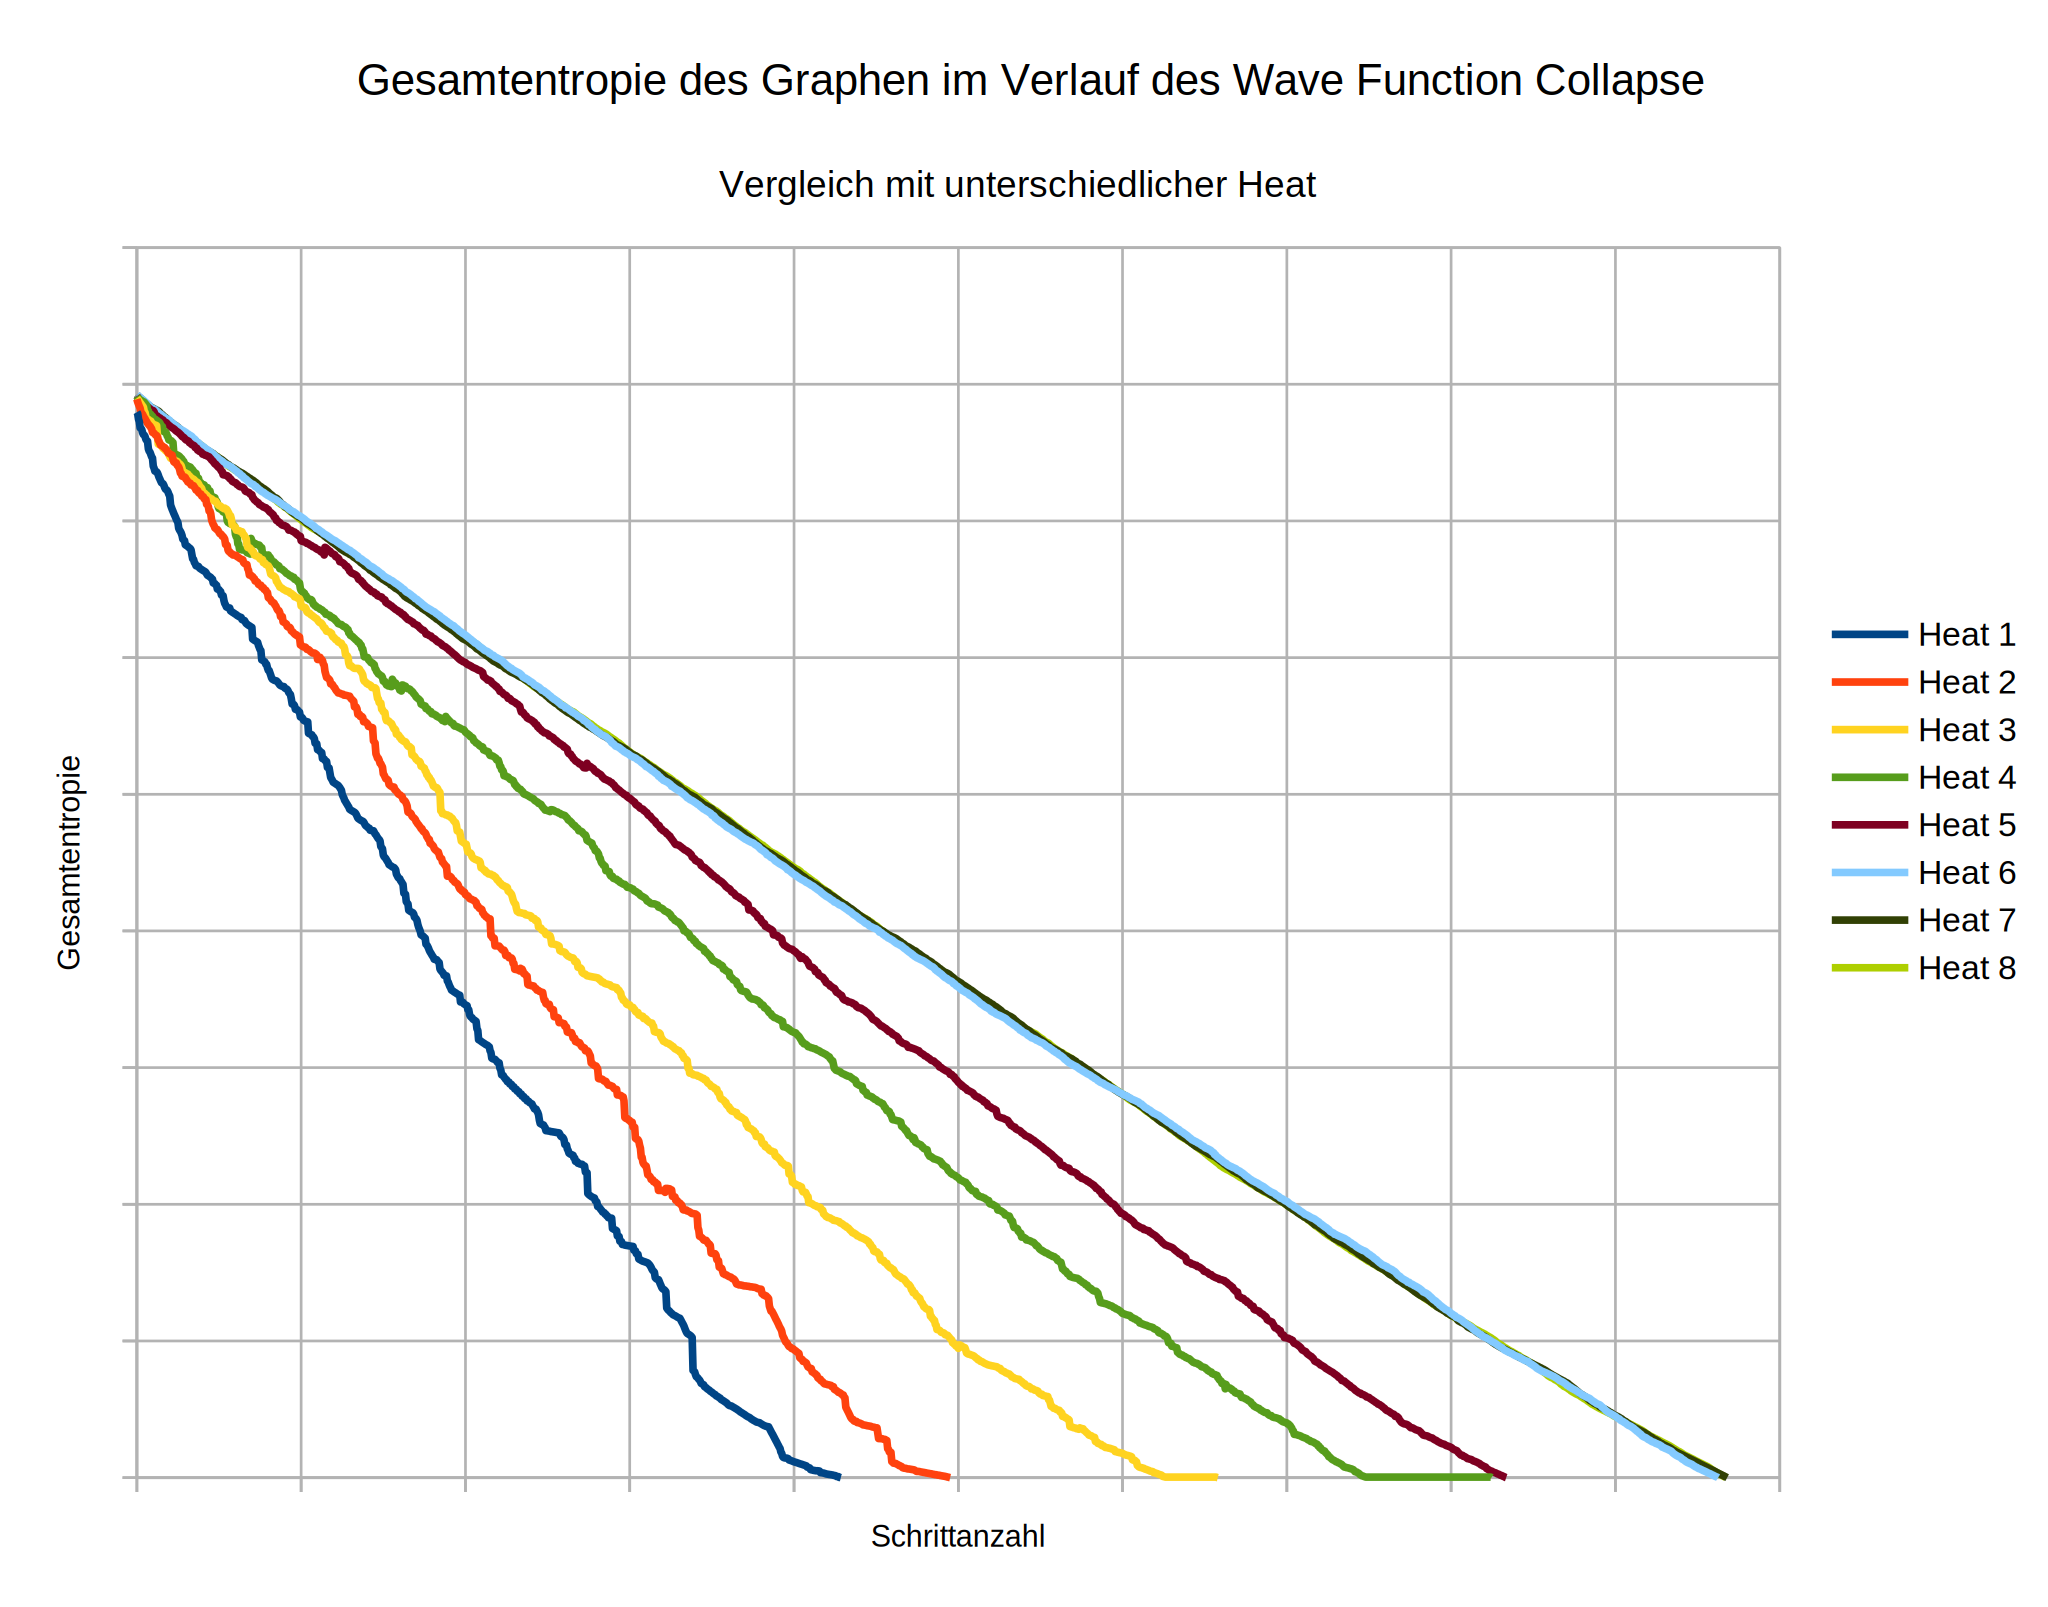
\includegraphics[width=\linewidth]{data/townscaper_grid/1.png} \caption{} \end{subfigure}
    \begin{subfigure}{0.18\textwidth} \includegraphics[width=\linewidth]{data/townscaper_grid/2.png} \caption{} \end{subfigure}
    \begin{subfigure}{0.18\textwidth} \includegraphics[width=\linewidth]{data/townscaper_grid/3.png} \caption{} \end{subfigure}
    \begin{subfigure}{0.18\textwidth} \includegraphics[width=\linewidth]{data/townscaper_grid/4.png} \caption{} \end{subfigure}
    \begin{subfigure}{0.18\textwidth} \includegraphics[width=\linewidth]{data/townscaper_grid/5.png} \caption{} \end{subfigure}
    
    \caption{
        Generierung eines Teils des Gitters für Townscaper \cite{stalberg_grid}. (a) Punkte werden generiert. (b) Triangulierung. (c) Kanten werden gelöscht, so dass Vierecke entstehen. (d) die Vierecke werden geviertelt. (e) Position der Knoten wird aufgelockert, so dass die Winkel zwischen Kanten gleichmäßiger sind.
    }
    \label{fig:townscaper_grid}
\end{figure}
        
    \subsection{Heat}
        \at{@incomplete introduction and definition}
        
        In einem 2D Gitter sind die Nachbarn jeder Zelle per Definition des Gitters in festen Richtungen und Abständen zu finden. Bei Graphen ist diese Anordnung frei. Während der Propagate-Phase werden die möglichen Zustände von Nachbarzellen auf Überlappung geprüft. Ein Zustand einer Zelle ist möglich, wenn er mit mindestens einem Zustand jeder Nachbarzelle überlappen kann. Die Überlappung zweier Zustände hängt von der Richtung zwischen den Umfeldern der Zustände abhängt ab. Das heißt, dass für den Nachbar im Norden einer Zelle nur die Überlappung der Zustände im Norden relevant ist. Die Richtung zu einer Nachbarzelle auf einem Graphen wird als der Vektor vom Mittelpunkt der Zelle zum Mittelpunkt der Nachbarzelle definiert. Der wichtigste Unterschied ist, dass die Richtung nun nicht mehr auf die acht Himmelsrichtungen (N, NO, O, SO, S, SW, W, NW) beschränkt ist. 
        
        Es ist nicht möglich Regeln für eine beliebige Richtung aus dem Beispiel zu extrahieren, da jeder Pixel nur 8 angrenzende Pixel hat. Sieht man das Beispiel als eine Funktion an, so ist diese nicht an allen Punkten definiert \at{(@incomplete Bilder als diskreten oder kontinuierliche Funktionen)}. Man könnte durch Interpolation einen Mittelwert zwischen gegebenen Werten berechnen, wenn das Bild eine kontinuierliche Funktion approximiert. Handelt es sich aber tatsächlich um eine diskrete Funktion, würde eine Interpolation Werte ergeben die vielleicht nicht Teil des Wertebereichs waren, in anderen Worten würde man Farbwerte erhalten die vorher nicht im Bild waren. Da die Ausgabe dem Beispiel ähnlich seien muss, entfällt diese Option.
        
        Es bleibt also nur die Möglichkeit, dass der tatsächlichen Richtung eine der messbaren Himmelsrichtungen zugewiesen wird. Hierfür wird die Kosinus-Ähnlichkeit \cite{cosine} \ref{fig:cosine} berechnet. Es wird die Himmelsrichtung mit der höchsten Ähnlichkeit gewählt. \at{@incomplete Kann auch mehr als eine Richtung sein}. \at{@incomplete Globale Heat}
        
        \begin{figure}[H]
    \centering
    
    $$ \mathrm{similarity}(\mathbf{a},\mathbf{b}) = \frac{\mathbf{a}\cdot\mathbf{b}}{\|\mathbf{a}\|_2\,\|\mathbf{b}\|_2} $$
    
    \caption{Formel für die Kosinus-Ähnlichkeit}
    
    \label{fig:cosine}
\end{figure}






\section{Umsetzung}
    \at{@incomplete Einleitender Satz}
    
    \subsection{Generierung von Graphen \at{@naming}}
        \at{@flow}
        \at{@flow}
        \at{@flow}
        \at{@flow}
        \at{@flow}
        
        Für den Algorithmus ist es egal, auf welche Weise der Graph erstellt wurde. Da der Fokus dieser Arbeit nicht in der Generierung von Graphen lag, habe ich mich auf einen Ablauf beschränkt. Es wird eine Menge an Punkten erstellt, darauf wird eine Delaunay-Triangulierung generiert, welche den Graphen darstellt. Gleichzeitig ist der duale Graph einer solchen Triangulierung ein Voronoi-Diagramm, welches zur Darstellung für den Nutzer verwendet wurde.
        
        \at{@placement nochmal überdenken}
        Man kann ein regelmäßiges Quadratgitter als eine spezielle Form von Voronoigraph ansehen. Jedes Quadrat kann als eine Voronoizelle angesehen werden, welche genau alle Punkte die am nächsten zu seinem Mittelpunkt enthällt. Die Nachbarn können nun explizit über die Kanten der Voronoizelle gefunden werden. Zuvor waren diese auch implizit durch die Koordinate des Quadrats im Gitter gegeben. Für den Algorithmus ist diese Unterscheidung egal und er generiert die gleiche Art von Ausgaben ohne weitere Anpassungen. \at{@visual} 
        
        \at{@incomplete Mehr zu diesem Prozess }
        \at{@incomplete Delaunay und Bowyer-Watson \cite{bowyer} \cite{watson}}
        \at{@incomplete Voronoi}
        \at{@incomplete welche Settings gibt einem die App dafür}\at{@visual Beispiele der Generierung}
        \at{@visual Delaunay Triangulierung und Voronoi Diagramme, dualer Graph}
        \at{@visual \ref{fig:graph_gen}}
        \at{@visual \ref{fig:voronoi_clipping}}
        % @todo(viktor): reihenfolge
        \begin{algorithm}
    \caption{Generierung eines Graphen}
    \label{alg:graph_gen}
        
    \begin{enumerate}
    \item Erstelle eine Menge an Punkten
    
    \item Generiere die Delaunay-Triangulierung der Punkte
    \subitem Die Ecken und Kanten aller Dreiecke bilden den Graphen
        
    \item Erstelle die Voronoi-Zellen aus der Triangulierung \begin{enumerate}
        \item Finde alle Dreiecke, die einen Punkt teilen
        \item Die Schwerpunkte dieser Dreiecke sind die Eckpunkte der Zelle
        \item Verbinde die Eckpunkte der Zelle mit Kanten
        \item Begrenze die Voronoi-Zellen auf den gewünschten Bereich 
        \subitem siehe Abbildung \ref{fig:voronoi_clipping}
        \end{enumerate}
    \end{enumerate}
        
\end{algorithm} % @todo(viktor): reference this
        \begin{figure}[H]
    \centering
    \begin{subfigure}{0.18\textwidth} 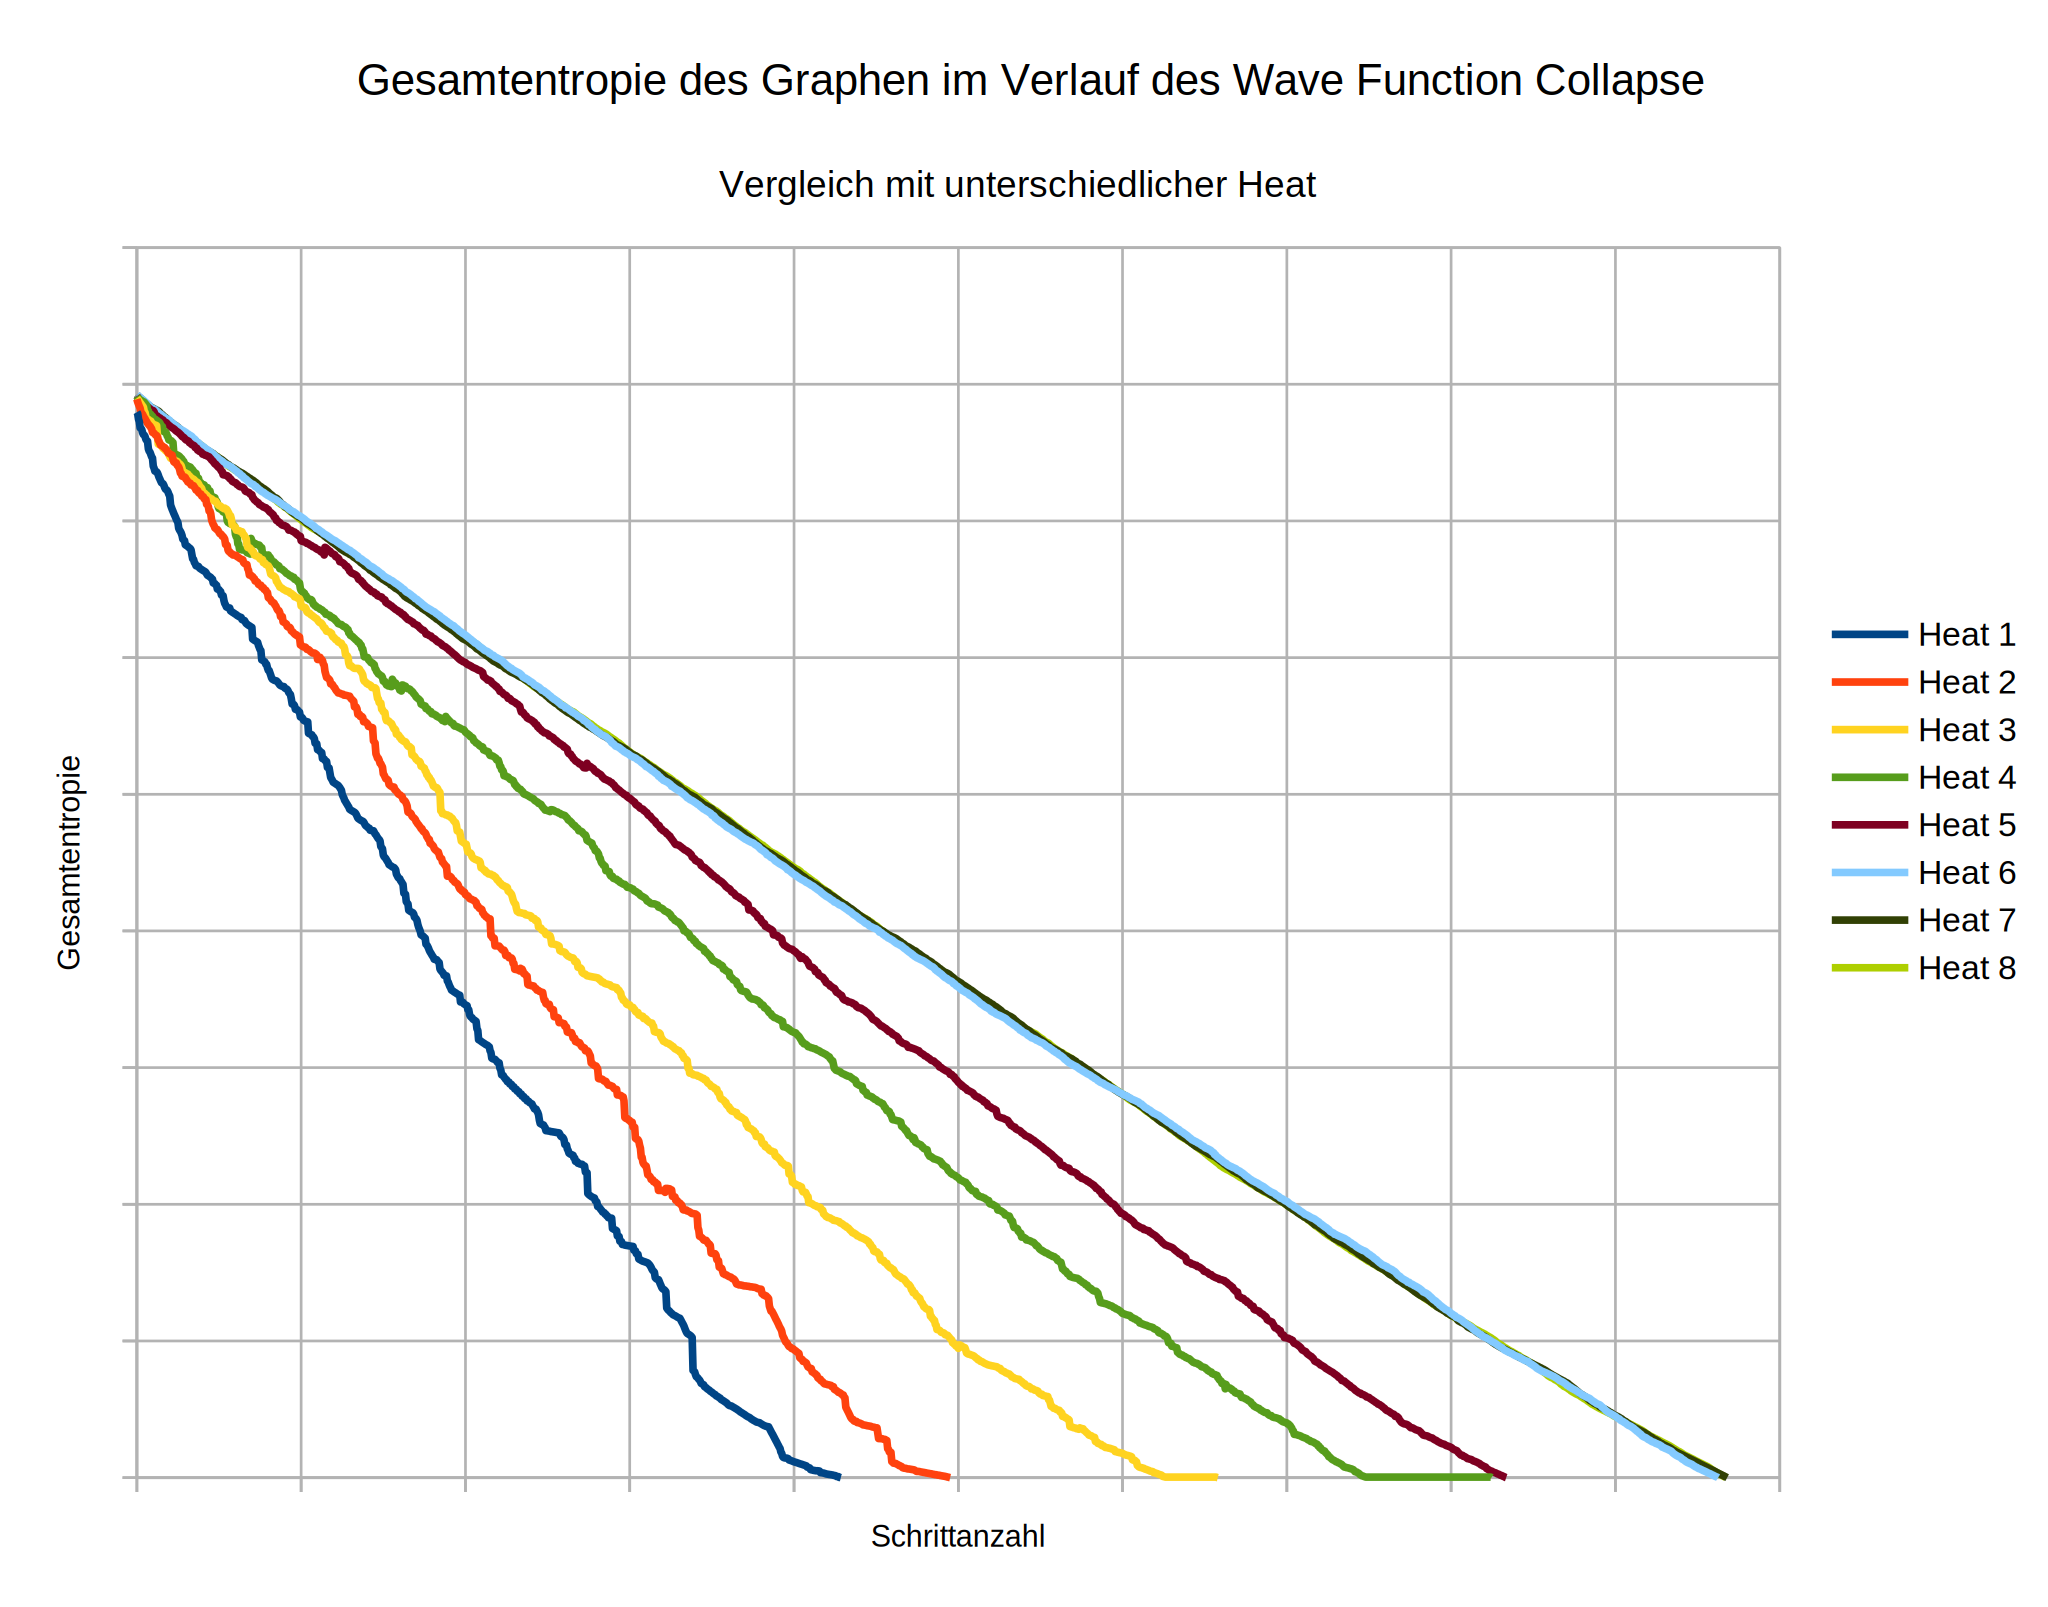
\includegraphics[width=\linewidth]{data/townscaper_grid/1.png} \caption{} \end{subfigure}
    \begin{subfigure}{0.18\textwidth} \includegraphics[width=\linewidth]{data/townscaper_grid/2.png} \caption{} \end{subfigure}
    \begin{subfigure}{0.18\textwidth} \includegraphics[width=\linewidth]{data/townscaper_grid/3.png} \caption{} \end{subfigure}
    \begin{subfigure}{0.18\textwidth} \includegraphics[width=\linewidth]{data/townscaper_grid/4.png} \caption{} \end{subfigure}
    \begin{subfigure}{0.18\textwidth} \includegraphics[width=\linewidth]{data/townscaper_grid/5.png} \caption{} \end{subfigure}
    
    \caption{
        Generierung eines Teils des Gitters für Townscaper \cite{stalberg_grid}. (a) Punkte werden generiert. (b) Triangulierung. (c) Kanten werden gelöscht, so dass Vierecke entstehen. (d) die Vierecke werden geviertelt. (e) Position der Knoten wird aufgelockert, so dass die Winkel zwischen Kanten gleichmäßiger sind.
    }
    \label{fig:townscaper_grid}
\end{figure}
        
        
        \subsubsection{Generierung von Voronoi-Graphen}
            Für die Triangulierung habe ich mich ohne tiefere Beweggründe für den Boywer-Watson Algorithmus entschieden. Der Algorithmus generiert die Triangulierung iterativ in dem jeder Punkt nacheinander eingefügt wird und der Graph angepasst wird, so dass es wieder eine Delaunay-Triangulierung ist.
            Zur Hilfe erstellen wir ein Superdreieck, welches alle Punkte enthällt. Nun fügen wir einen Punkt ein und prüfen all bisher gefundenen Dreiecke, ob ihr Umkreis diesen Punkt enhällt. Ist der Punkt innerhalb des Umkreises kann das Dreieck nicht zur finalen Triangulierung gehören. Für alle diese Dreieck sammeln wir nun die Kanten. Jede Kante die nur einmal vorkommt ist teil der Hülle dieser Dreiecke, alle anderen Kanten sind innerhalb dieser Hülle, da sich zwei Dreiecke diese teilen. Diese inneren Kanten werden entfernt und für jede Ecke entlang der Hülle wird eine neue Kante zum eingefügten Punkt erstellt.
            Am Ende entfernt alle Kanten zur den Eckpunkten des Superdreiecks aus der Triangulierung und erhällt die Delaunay-Triagulierung der Point-Cloud.
            
            Aus der Triangulierung erstellen wir das Voronoidiagram indem wir die Eckpunkte als Mittelpunkte der Voronoizellen nehmen. Die Kanten sagen uns welche Zellen benachbart sind. Um die Kanten der Voronoizelle zu finden nehmen wir von alle Dreiecke in denen der Punkt liegt den Mittelpunkt des Umkreises. Die Umkreismittelpunkte sind die Ecken der Voronoizelle. Die Kanten finden wir indem wir die Punkte nach ihrem Winkel um den Mittelpunkt der Zelle sortieren und dann der Reihe nach verbinden.
            
            Es ist normal, dass ein solches Voronoidiagram an den Rändern der Point-Cloud auch Zellen ergeben kann die auf einer Seite offen sind, weil die Kanten zwischen den Ecken der Zelle, den Umkreismittelpunkten, keinen Schnittpunkt haben. Ich habe mich dazu entschieden, bei solchen Zellen weitere Eckpunkte einzufügen, so dass das alle Zellen durch einen freigewählten rechteckigem Bereich begrenzt sind. Dafür prüfe ich ob ein Eckpunkt außerhalb des Bereichs liegt und finde dann den Schnittpunkt von der Kante zu dem Eckpunkt mit dem Rechteck des Bereichs und ersetze den Eckpunkt mit diesem Schnittpunkt. Dieser Schritt passiert so lange bis alle Eckpunkte innerhalb oder auf dem Rand des Bereichs liegen.
                Siehe Abbildung \ref{fig:voronoi_clipping}.



    \subsection{Phasen \at{@naming}}
        Der Algorithmus \ref{fig:wfc_back} generiert die Ausgabe schrittweise. Ein Schritt kann in vier Phasen geteilt werden: Search, Pick, Observe und Propagate.
        
        \begin{figure}[H]
    \centering
    \begin{minipage}{\linewidth}
        \rule{\linewidth}{0.4pt}
        
        \begin{enumerate}
            \item Führe den nächsten \textbf{Schritt} aus: \begin{enumerate}
                \item \textbf{Search}: Finde die Zellen mit der geringsten Entropie \begin{enumerate}
                    \item Sind alle Zellen kollabiert? $\rightarrow$ \textbf{Done}
                    \item Erstelle ein Liste der gefundenen Zellen
                \end{enumerate}
                
                \item \textbf{Pick}: Wähle eine Zelle aus \begin{enumerate}
                    \item Ist die Liste der Zellen leer? $\rightarrow$ \textbf{Backtrack}
                    \item Entferne die gewählte Zelle aus der Liste
                    \item Notiere alle möglichen Zustände der Zelle in einer Liste
                \end{enumerate}
                
                \item \textbf{Observe}: Wähle einen Zustand aus \begin{enumerate}
                    \item Entferne den gewählten Zustand aus der Liste
                    \item Kollabier die Zelle in den Zustand
                    \item Ist die Liste der Zustände leer? $\rightarrow$ \textbf{Backtrack}
                \end{enumerate}
                
                \item \textbf{Propagate}: Prüfe alle Nachbarn von geänderten Zellen \begin{enumerate}
                    \item Erstelle eine Liste zu prüfender Zellen
                    \item Füge die ausgewählte Zelle ein
                    \item Prüfe alle Nachbarzellen ob ihre Zustände noch passen
                    \item Füge die Nachbarn in die Liste ein, wenn sie sich verändert haben
                    \item Hat die Nachbarzelle keine möglichen Zustände mehr? $\rightarrow$ \textbf{Backtrack}
                \end{enumerate}
                
                \item Geh zum nächsten \textbf{Schritt}
            \end{enumerate}
            \item \textbf{Backtrack}: \begin{enumerate}
                \item Gehe zum gewünschten Schritt zurück
                \item Gehe eine Phase in dem Schritt zurück
                \item Füge alle Zustände aller Zellen, dessen Entfernungsschritt nun nach dem aktuellen Schritt liegt, wieder in die Zelle ein
            \end{enumerate}
            \item \textbf{Done}: Gib das Resultat aus
        \end{enumerate}
            
        \rule{\linewidth}{0.4pt}
    \end{minipage}
    
    \caption{Wave Function Collapse mit Backtracking}
    
    \label{fig:wfc_back}
\end{figure} 
        
        Zu Beginn wird die Zelle mit der geringsten Entropie gesucht, die noch nicht collapsed ist. Die Entropie einer Zelle wird als die Shannon-Entropie \cite{shannon} der noch möglichen Zustände berechnet. Es ist möglich, dass mehrere Zellen die gleiche Entropie haben. Zum Beispiel sind alle Zellen am Anfang in der Superposition aller Zustände, wodurch alle Zellen die selbe Entropie haben. Aus der Menge an gefundenen Zellen wird in diesem Fall in der Pick-Phase eine Zelle zufällig ausgewählt.
        
        In der Observe-Phase wird ein Zustand aus der Superposition zufällig ausgewählt und die Zelle in diesen Zustand collapsed. Die anderen Zustände werden entfernt, was Einfluss auf die Nachbarzellen haben kann. Die Wahrscheinlichkeit eines Zustands, gewählt zu werden, hängt von dessen Häufigkeit im Beispiel ab. 
        
        Danach beginnt die Propagate-Phase. Eine Liste aller geänderten Zellen wird mit der observierten Zelle initialisiert. Jede Zelle in der Liste wird einzeln entfernt und wie folgt bearbeitet. Alle Nachbarzellen der betrachten Zellen prüfen, welche ihrer Zustände mit keinem der Zustände der betrachteten Zellen noch überlappen. Diese Zustände werden entfernt und jede Nachbarzelle die sich so verändert hat, wird der Liste angefügt. Sollte dabei auch der letzte mögliche Zustand einer Zelle unmöglich gewurden sein, so wurde ein Widerspruch erreicht; der Graph kann nun nicht mehr gelöst werden. Diese Phase dauert so lange, bis die Liste leer ist, sich also keine Zellen mehr verändern.
        
        
    \subsection{Backtracking}
        Wenn der Algorithmus einen Widerspruch entdeckt, muss nicht immer alle Arbeit verworfen werden. Gerade bei größeren oder komplizierteren Mustern oder Graphen ist es wahrscheinlich, dass beim ersten Versuch keine Lösung gefunden wird, weil die Komplexität den Lösungsraum stärker einschränkt. Wenn ein Widerspruch in einer Zelle aber nun nur von den direkten Nachbar abhängt, so ist es wahrscheinlich dass weiter entfernte bereits gelöste Zellen dennoch kompatibel sind. Um einen lokalen Widerspruch aufzulösen muss meistens nur lokal eine andere Entscheidung getroffen werden.
        
        Um Backtracking umzusetzen müssen mehr Informationen behalten werden als nur der Zustand des Gitters zum aktuellen Zeitpunkt. Will man nun wieder einen Schritt zurückgehen muss man wissen, welche Entscheidung man zuvor bereits getroffen hat um dessen Effekt rückgängig zu machen. Dabei genügt es nicht nur die collapste Zelle und den Zustand wieder zu entfernen, weil jede Zelle von mehreren Nachbarn beeinflusst wird. Die Zustandsmenge einer Zelle ist die Schnittmenge der möglichen Nachbarzuständen der Nachbar. Somit kann es sein, dass ein Zustand A aus der Menge wegen mehreren Einschränkungen von mehreren Nachbarn fehlt. Nimmt man nun durch Backtracking eine dieser Einschränkungen wieder zurück, so ist es nicht offensichtlich, ob Zustand A nun wieder möglich ist, ohne alle Einschränkungen auf die Zelle neu zu berechnen.
        Entweder man macht die Änderung nur lokal rückgängig und berechnet immer alle Zellen neu, bis sich keine mehr ändern. Oder man speichert ab, zu welchem Zeitpunkt ein Zustand unmöglich geworden ist und prüft ob dieser Zeitpunkt nach dem Schritt zurück weiterhin in der Vergangenheit oder nun in der Zukunft liegt. Bei zweiterem müssen alle solche Zustände als wieder möglich betrachtet werden.
        Diese Art die Menge an Zuständen darzustellen ist okay, weil sich für jede Zelle die Zustandsmenge in jedem Schritt des Algorithmus immer nur verkleinert oder gleichbleibt. Ist ein Zustand durch die Nachbar unmöglich so wird er auch nie wieder an späterem Zeitpunkt möglich.
        
        Desweiteren sollen bereits gemachte Entscheidungen, die zu einem Widerspruch führen, nicht noch einmal wiederholt werden. Die Entscheidungspunkte in der  Pick- und Observe-Phase können gleich behandelt werden. Wir können die List an Auswahlmöglichkeiten für später speichern und die ausgewählte Zelle oder den ausgewählten Zustand von der Liste entfernen. Wird auf einen Schritt gebacktrackt, so kann einfach die nächste Möglichkeit auswählt werden. Der Algorithmus läuft ab dann normal weiter .In der Umsetzung wird für jede Zelle eine Liste aller Zustände gespeichert. Jeder Zustand ist entweder möglich und wurde noch nicht entfernt oder ist unmöglich und speichert den Zeitpunkt an dem er unmöglich wurde. Hierbei ist der Zeitpunkt einfach die Nummer des Schritts an dem der Zustand unmöglich wurde. 
        
        \at{@placement}
        Der Algorithmus ist in Abbildung \ref{fig:wfc_back} dargestellt. Für jeden Schritt des Algorithmus wird auch die Liste der gefundenen Zellen in der Search-Phase gespeichert. Wenn in der Pick-Phase eine Zelle ausgewählt wird, wird diese aus der Liste entfernt, damit diese beim Backtracken nicht erneut gewählt wird. Ebenso werden in der Observe-Phase alle wählbaren Zustände gespeichert und mit jedem Lösungsversuch wird der gewählte Zustand entfernt. Nun wurde aber eine Schwachstelle in den Algorithmus eingeführt. Wenn zuvor in der Search-Phase keine Zellen in Superposition mehr gefunden wurden, bedeutete dies, dass alle Zellen tatsächlich collapsed waren. Nun kann es sein, dass alle Zellen, die gefunden wurden, zu einem Widerspruch führen würden und entfernt wurden. Somit würde keine Zelle mehr wählbar sein. Auch in der Observe-Phase war es zuvor unmöglich keinen Zustand mehr auswählen zu können, da eine Zelle mit leerer Zustandsmenge bereits zuvor als Widerspruch identifiziert wurden wäre. In diesen Fällen wurde ein Widerspruch erreicht und es muss zum Backtracking kommen. Schließlich wurden alle noch möglichen Entscheidungen bereits getroffen und ausgewertet und keine Lösung gefunden. Somit führt dieser Schritt zwar nicht direkt zu einem Widerspruch in einer Zelle, aber alle folgen Schritte werden irgendwann zu einem Widerspruch führen. Als Anmerkung: wird auf diese Weise bis zum ersten Schritt gebacktrackt und führen dann auch dort alle möglichen Entscheidungen zu einem Widerspruch, so kann die Kombination aus Beispiel und Graph keine Ausgabe ergeben.
        
    \subsection{Überlappung und Heat \at{@naming}}
        \at{@incomplete was muss zur implementierung gesagt werden, was nicht schon an anderer stelle ein zuhause gefunden hat}





\section{Ergebnisse}
    \at{@incomplete Einleitender Satz}
    
    \begin{itemize}
    \item Base Case - Gitter
    \item Bilder mit unterschiedlichen Graphen: Einfache, Komposition(vier in eins, außen und innen)
    \end{itemize}
    
    \subsection{Der Effekt von Heat auf die Ausgabe}
        \at{@incomplete introduction}
        
        
        Abbildung \ref{fig:hex_heat} zeigt den Einfluss von Heat auf die Qualität der Ausgabe bei gleichem Beispiel und Graph. Das Beispiel kann auf dem Quadratgitter ohne weitere Probleme genutzt werden, während der Graph mit den Sechsecken bei geringer Heat uninteressante Ausgaben generiert. \at{@incomplete (a) erwähnen}
        
        \begin{figure}[H]
    \centering
    \begin{subfigure}{0.18\textwidth} 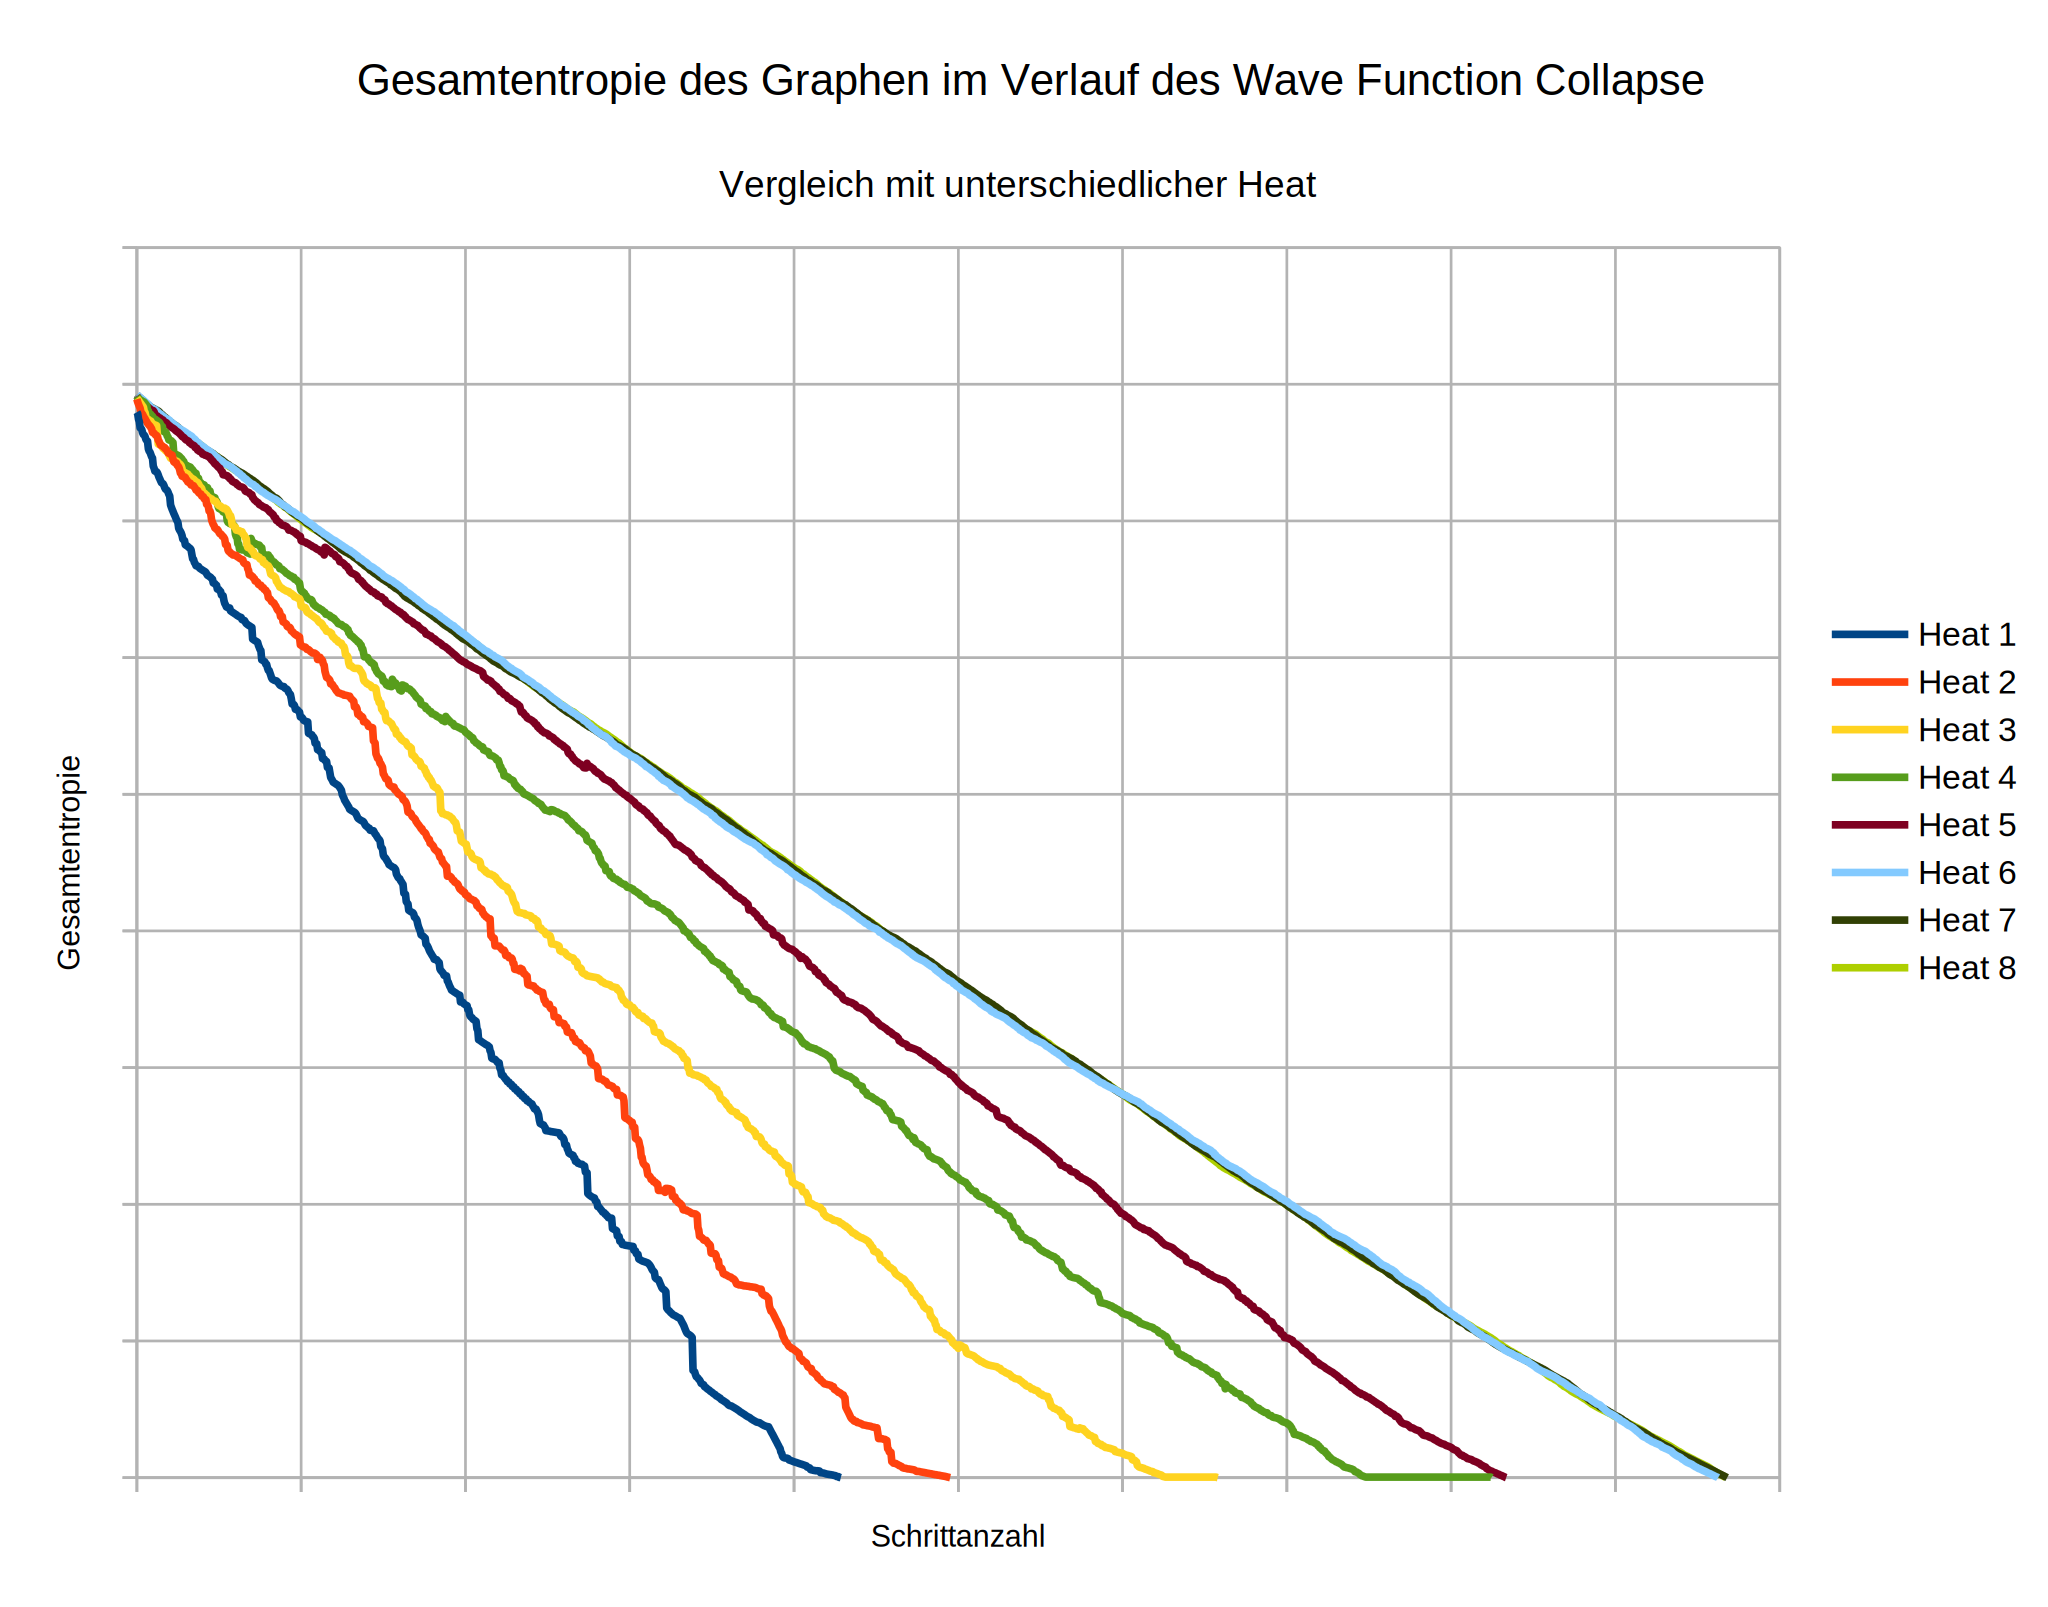
\includegraphics[width=\linewidth]{data/townscaper_grid/1.png} \caption{} \end{subfigure}
    \begin{subfigure}{0.18\textwidth} \includegraphics[width=\linewidth]{data/townscaper_grid/2.png} \caption{} \end{subfigure}
    \begin{subfigure}{0.18\textwidth} \includegraphics[width=\linewidth]{data/townscaper_grid/3.png} \caption{} \end{subfigure}
    \begin{subfigure}{0.18\textwidth} \includegraphics[width=\linewidth]{data/townscaper_grid/4.png} \caption{} \end{subfigure}
    \begin{subfigure}{0.18\textwidth} \includegraphics[width=\linewidth]{data/townscaper_grid/5.png} \caption{} \end{subfigure}
    
    \caption{
        Generierung eines Teils des Gitters für Townscaper \cite{stalberg_grid}. (a) Punkte werden generiert. (b) Triangulierung. (c) Kanten werden gelöscht, so dass Vierecke entstehen. (d) die Vierecke werden geviertelt. (e) Position der Knoten wird aufgelockert, so dass die Winkel zwischen Kanten gleichmäßiger sind.
    }
    \label{fig:townscaper_grid}
\end{figure}
        
        Die intuitive Erklärung ist, dass die Linien im Beispiel stets nur eine Zelle breit sind. Im Graph können die horizontalen Linien generiert werden, weil die Sechsecke selbst horizontal in Reihen angeordnet sind, während es keine rein vertikalen Zellenspalten gibt. Jedes Sechseck hat zwei Nachbarzellen oberhalb und zwei unterhalb. Bei Heat=1 wird beiden Norden/Süden zugewiesen. Will der Algoritmus nun bei einer Zelle eine vertikalen Linie, also die Zustände die dieses Muster abbilden, platzieren, so müssen nun beide oberen Nachbarzellen auch eine Zustand, der eine vertikale Linie darstellt, erhalten. Hier kommt es zum Konflikt, da diese beiden Zellen horizontal in der gleichen Reihe liegen, es aber im Beispiel keine vertikalen Linien direkt nebeneinander gibt. Es kann also keine Zelle Teil einer vertikalen Linie sein. 
        
        Bei (c) können dennoch \textbf{scheinbar} vertikale Linien generiert werden, da nun die oberen Zellen jeweils als im Norden und imd Nordosten/-westen betrachtet werden. Ebenso können die horizontalen Nachbarn als im Westen oder im Süd-/Nord-westen behandelt werden. Soll eine Zelle nun Teil einer vertikalen Linie sein, kann nur eine der oberen Nachbarnzellen als im Norden behandelt werden und die andere als die jeweilige Diagonale. 
        
        \at{@incomplete Entropie erwähnen} Der Effekt von höherer Heat ist, das die Menge an möglichen Zuständen vergrößert wird, indem mehr Überlappungsregeln in Betracht gezogen werden. Dadurch ist es auch unwahrscheinlicher, dass für eine Zelle keine Zustände mehr möglich sind und ein Widerspruch entsteht. Gleichzeitig werden nun aber auch Ausgaben generiert, die eine tatsächlich geringere Ähnlickkeit zum Beispiel haben. So ist die Ausgabe in (b) zwar weniger interessant als die in (c), aber die horizontalen Linien und die grauen Flächen dazwischen passen exakt zur Teilen des Beispiels. Bei (c) werden auch vertikalen Linien generiert, aber diese haben knicke und sind eher zickzackartig als die Senkrechten des Beispiels. Eine Erhöhung der Heat verschlechtert die lokale Ähnlichkeit der Ausgabe zum Beispiel und verbessert die Wahrscheinlichkeit erfolgreich eine nicht triviale Lösung zu generieren.
        
        In Abbildung \ref{fig:heat_rotation} ist dargestellt, wie Heat auch als eine lokale Drehung des Gitters verstanden werden kann. In (a) ist das gewählte Beispiel auf einem Quadratgitter ohne Drehung angewendet. Es können gute Ausgaben generiert werden. Dreht man das gesamte Quadratgitter nun um 22° so können die geraden Linien des Beispiels immernoch fehlerfrei platziert werden. Zwar sind die Zellen zueinander nicht mehr genau entlang der Himmelsrichtungen angeordnet, doch wird bei Heat=1 auf die nächste Richtung gerundet. Bei 8 Richtungen wird z.B. Osten von -22,5° bis 22,5° ausgewählt. Somit ist das Gitter bei (b) zwar optisch gedreht, aber kann genau wie das Gitter in (a) behandelt werden. Wird nun aber, wie in (c) noch weiter gedreht, so wird nun eine Benachbarung die vorher z.B. als Osten behandelt wurde nun als Nordosten behandelt. Der Effekt ist, dass die geradlinigen Muster des Beispiels nun (wie zuvor bei Abbildung \ref{fig:hex_heat}) nicht mehr platziert werden können. In der Ausgabe können nur noch flächenartige Muster vorkommen. In (d) ist zu sehen, dass dennoch gute Ausgaben generiert werden können, indem die Heat=2 gesetzt wird und jede Benachbarung nun z.B. als Nordosten und Osten behandelt wird. Der Algorithmus kann nun Ausgaben wie bei (b) generieren, da die Benachbarungen nun auch lokal wie die Benachbarungen aus (a) und (b) behandelt werden können. Heat kann also auch als eine lokale Drehung entgegen der tatsächlichen Ausrichtung des Gitters wirken. 
        
        \begin{figure}[H]
    \centering
    \begin{subfigure}{0.18\textwidth} 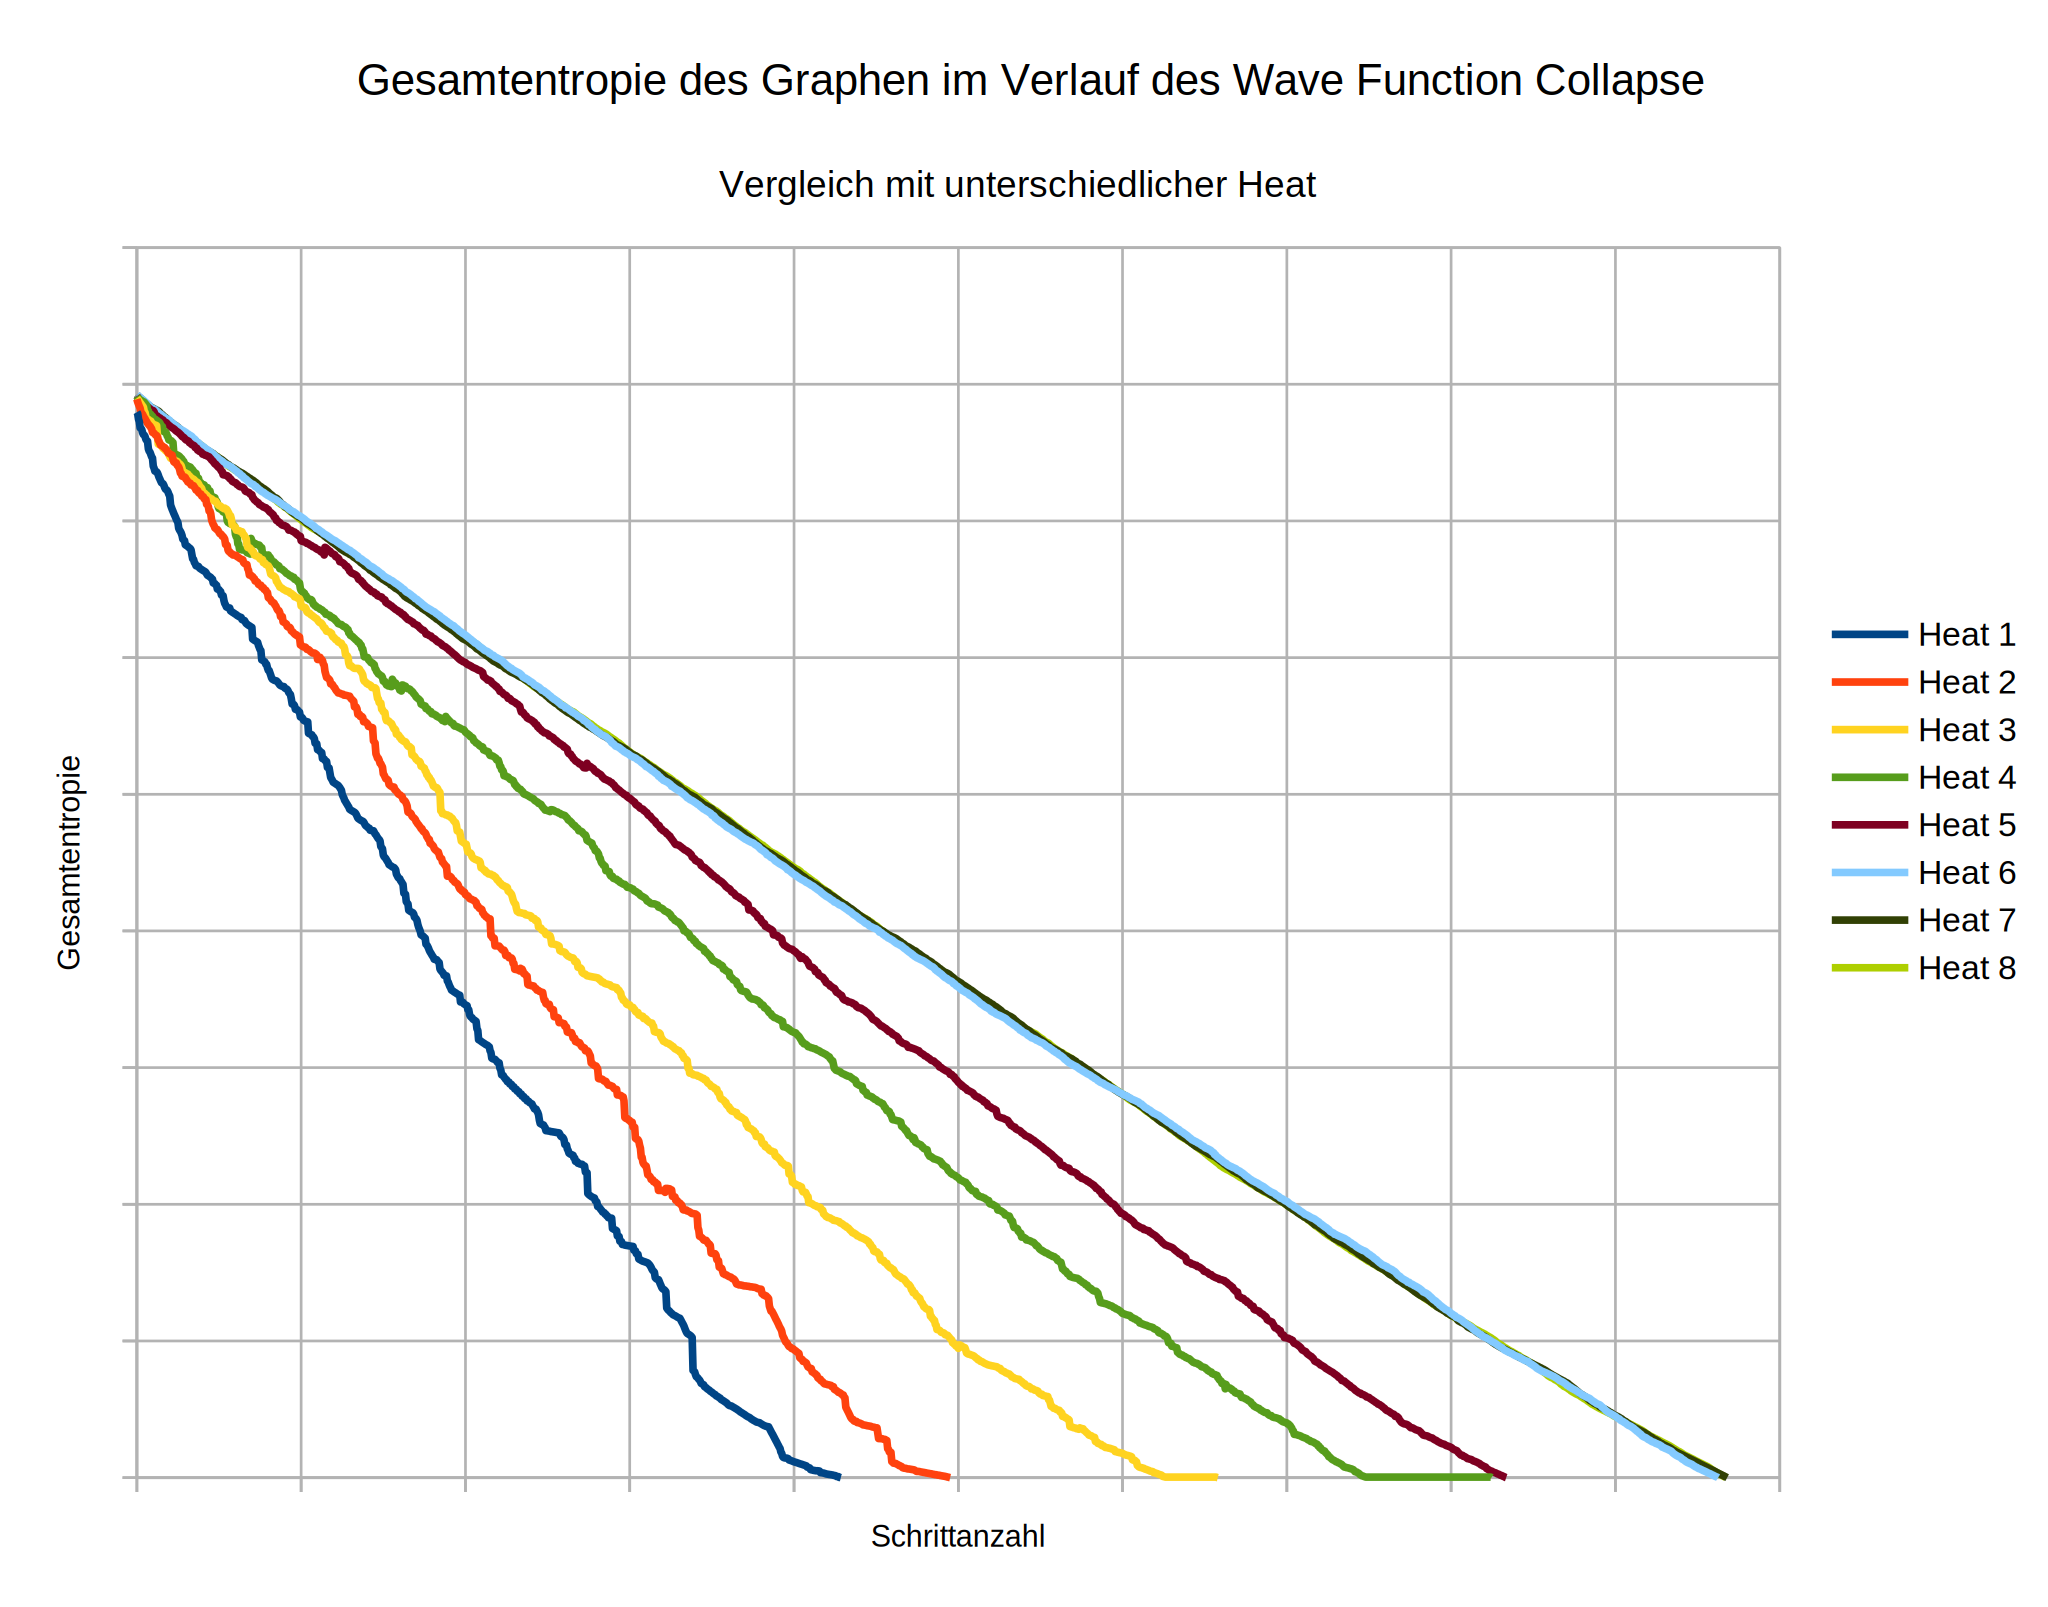
\includegraphics[width=\linewidth]{data/townscaper_grid/1.png} \caption{} \end{subfigure}
    \begin{subfigure}{0.18\textwidth} \includegraphics[width=\linewidth]{data/townscaper_grid/2.png} \caption{} \end{subfigure}
    \begin{subfigure}{0.18\textwidth} \includegraphics[width=\linewidth]{data/townscaper_grid/3.png} \caption{} \end{subfigure}
    \begin{subfigure}{0.18\textwidth} \includegraphics[width=\linewidth]{data/townscaper_grid/4.png} \caption{} \end{subfigure}
    \begin{subfigure}{0.18\textwidth} \includegraphics[width=\linewidth]{data/townscaper_grid/5.png} \caption{} \end{subfigure}
    
    \caption{
        Generierung eines Teils des Gitters für Townscaper \cite{stalberg_grid}. (a) Punkte werden generiert. (b) Triangulierung. (c) Kanten werden gelöscht, so dass Vierecke entstehen. (d) die Vierecke werden geviertelt. (e) Position der Knoten wird aufgelockert, so dass die Winkel zwischen Kanten gleichmäßiger sind.
    }
    \label{fig:townscaper_grid}
\end{figure}
        
        Der selbe Effekt kommt auch bei unregelmäßigen Graphen zum Spiel. Hier existiert zwar kein Winkel um den man den gesamten Graphen drehen kann, um ein Quadratgitter zu erhalten. Aber da Heat lokal und von Nachbar zu Nachbar unabhängig wirkt, kann es als eine lokale Drehung oder Verzerrung verstanden werden. Es ist so, als könnte der Algorithmus die Zellen lokal so verschieben und verdrehen, dass einen breitere Menge an Lösungen möglich ist. Es muss dabei beachtet werden, dass der Algorithmus nicht gezielt arbeitet. Ist eine Graph bereits mit geringer Heat gut lösbar, so wird höhere Heat nicht unbedingt auch bessere Ergebnisse liefern. Es ist sogar wahrscheinlich, dass die Ausgabe schlechter wird da die höhere Heat ja auch zu Regionen in der Ausgabe führt die nicht im Beispiel existieren und den Einfluss der Richtung mindert.
        
        Abbildung \ref{fig:more_heat} zeigt wie die Qualität der Ausgabe, bei steigender Heat, sinken kann. Der Graph ist hier ein Quadratgitter und kann somit schon bei einer Heat von 1 gute Ausgaben generieren. Mit jedem Schritt wird der jeder tatsächlichen Benachbarung eine größere Menge an Möglichkeiten gegeben. Es entstehen mehr fehlerhafte Regionen in der Ausgabe. Ab einer Heat von 5 kann der Algorithmus einer perfekt nach Osten laufenden Benachbarung nicht nur Nordosten und Südosten sondern auch Norden und Süden zuweisen, also zu einander entgegengesetzte Himmelrichtgen. Liegt z.B. eine Zelle östlich von einer anderen so könnten beide sich als südlich der anderen behandeln. Ab Heat=6 könnte jede Benachbarung auch als eine der entgegengesetze Himmelrichtungen behandelt werden. Schließlich verliert die Anordnung der Zellen bei Heat=8 komplett die Bedeutung. Zur Vollständigkeit sind hier Ausgaben mit hoher Heat dargestellt, in der Praxis sollte man Heat so gering wie möglich halten.
        
        \begin{figure}[H]
    \centering
    \begin{subfigure}{0.18\textwidth} 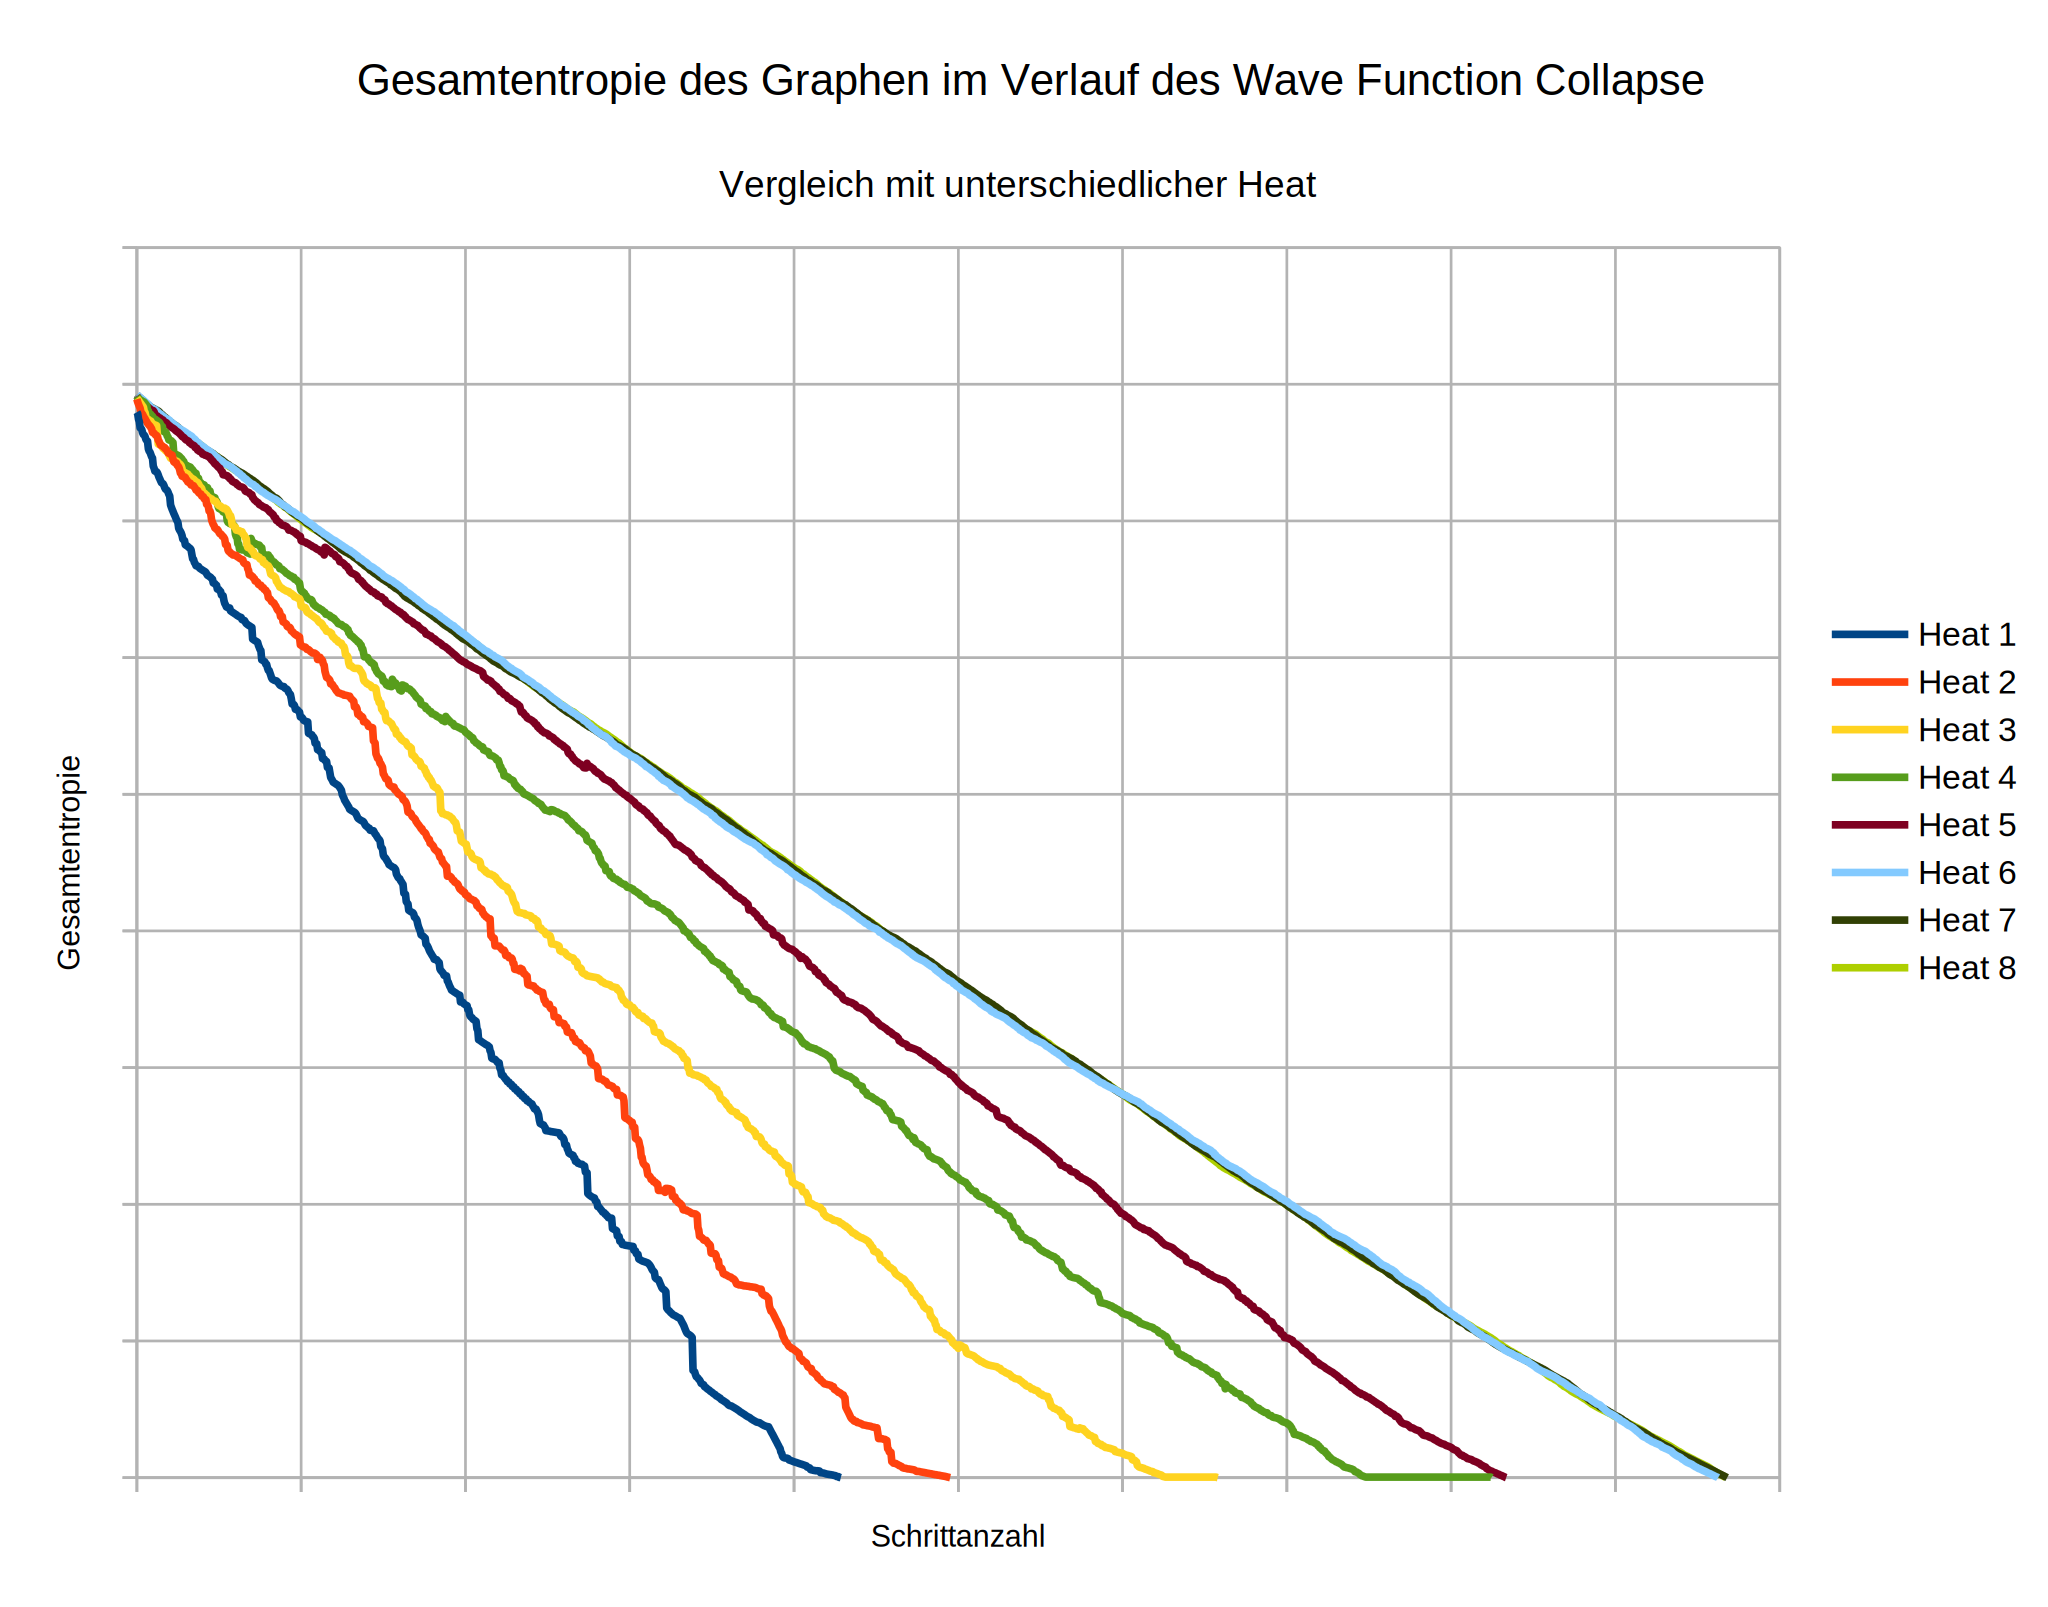
\includegraphics[width=\linewidth]{data/townscaper_grid/1.png} \caption{} \end{subfigure}
    \begin{subfigure}{0.18\textwidth} \includegraphics[width=\linewidth]{data/townscaper_grid/2.png} \caption{} \end{subfigure}
    \begin{subfigure}{0.18\textwidth} \includegraphics[width=\linewidth]{data/townscaper_grid/3.png} \caption{} \end{subfigure}
    \begin{subfigure}{0.18\textwidth} \includegraphics[width=\linewidth]{data/townscaper_grid/4.png} \caption{} \end{subfigure}
    \begin{subfigure}{0.18\textwidth} \includegraphics[width=\linewidth]{data/townscaper_grid/5.png} \caption{} \end{subfigure}
    
    \caption{
        Generierung eines Teils des Gitters für Townscaper \cite{stalberg_grid}. (a) Punkte werden generiert. (b) Triangulierung. (c) Kanten werden gelöscht, so dass Vierecke entstehen. (d) die Vierecke werden geviertelt. (e) Position der Knoten wird aufgelockert, so dass die Winkel zwischen Kanten gleichmäßiger sind.
    }
    \label{fig:townscaper_grid}
\end{figure}





\section{Diskussion}
    \at{@incomplete Einleitender Satz}
    
    \begin{itemize}
    \item Vergleich zum WFC, wie und was vergleichen?
    \item Lokale Ähnlichkeit im Vergleich zum Input
    \item Linienmuster und Flächenmuster  in Beispielen
    \end{itemize}





\section{Fazit - Ausblick und zukünftige Forschung \at{@naming}}
    \begin{itemize}
    \item Mögliche Anwendungsbereiche
    \item WFC auf 3D Graphen
    \item Eigenschaften des Musters(Linien und Flächen) in Bezug auf Heat
    \item Eigenschaften des Gitters analysieren, Engpässe, unförmige Zellen, Abstände, Form der Zelle beachten
    \end{itemize}
    
    \subsection{Heat}
        \begin{itemize}
        \item Eine globale Heat für alle Zellen hat einen negativen Effekt auf lokal regelmäßige Regionen eines Gitters und ein postiven Effekt auf sehr unregelmäßige Regionen des Gitters.
        \item Anstatt dass die Heat global für alle Zellen zu Beginn bestimmt wird, kann man auch während des Collapse 'lernen' welche Regionen 'schwerer' zu lösen sind und dort die Heat schrittweise erhöhen bis eine Lösung gefunden werden kann.
        \item Lokales Heating mit heating chance und cooling chance
        \item simmulated annealing
        \end{itemize}





% ////////////////////////////////////////////////
% ////////////////////////////////////////////////

\@todo(viktor):{quellen für delaunay-triangulation und voronoi-diagrams}

\pagebreak
\bibliographystyle{plain}
\bibliography{Literatur}

\end{document}